\setchapterstyle{lines}
\labch{appendix}

\setchapterstyle{lines}
\chapter{Heavy Neutral Lepton Signal Simulation}
\labch{signal_simulation_appenix}


\section{Model Independent Simulation Distributions} \labsec{model_independent_simulation_appendix}

\begin{figure*}[h]
    \centering
    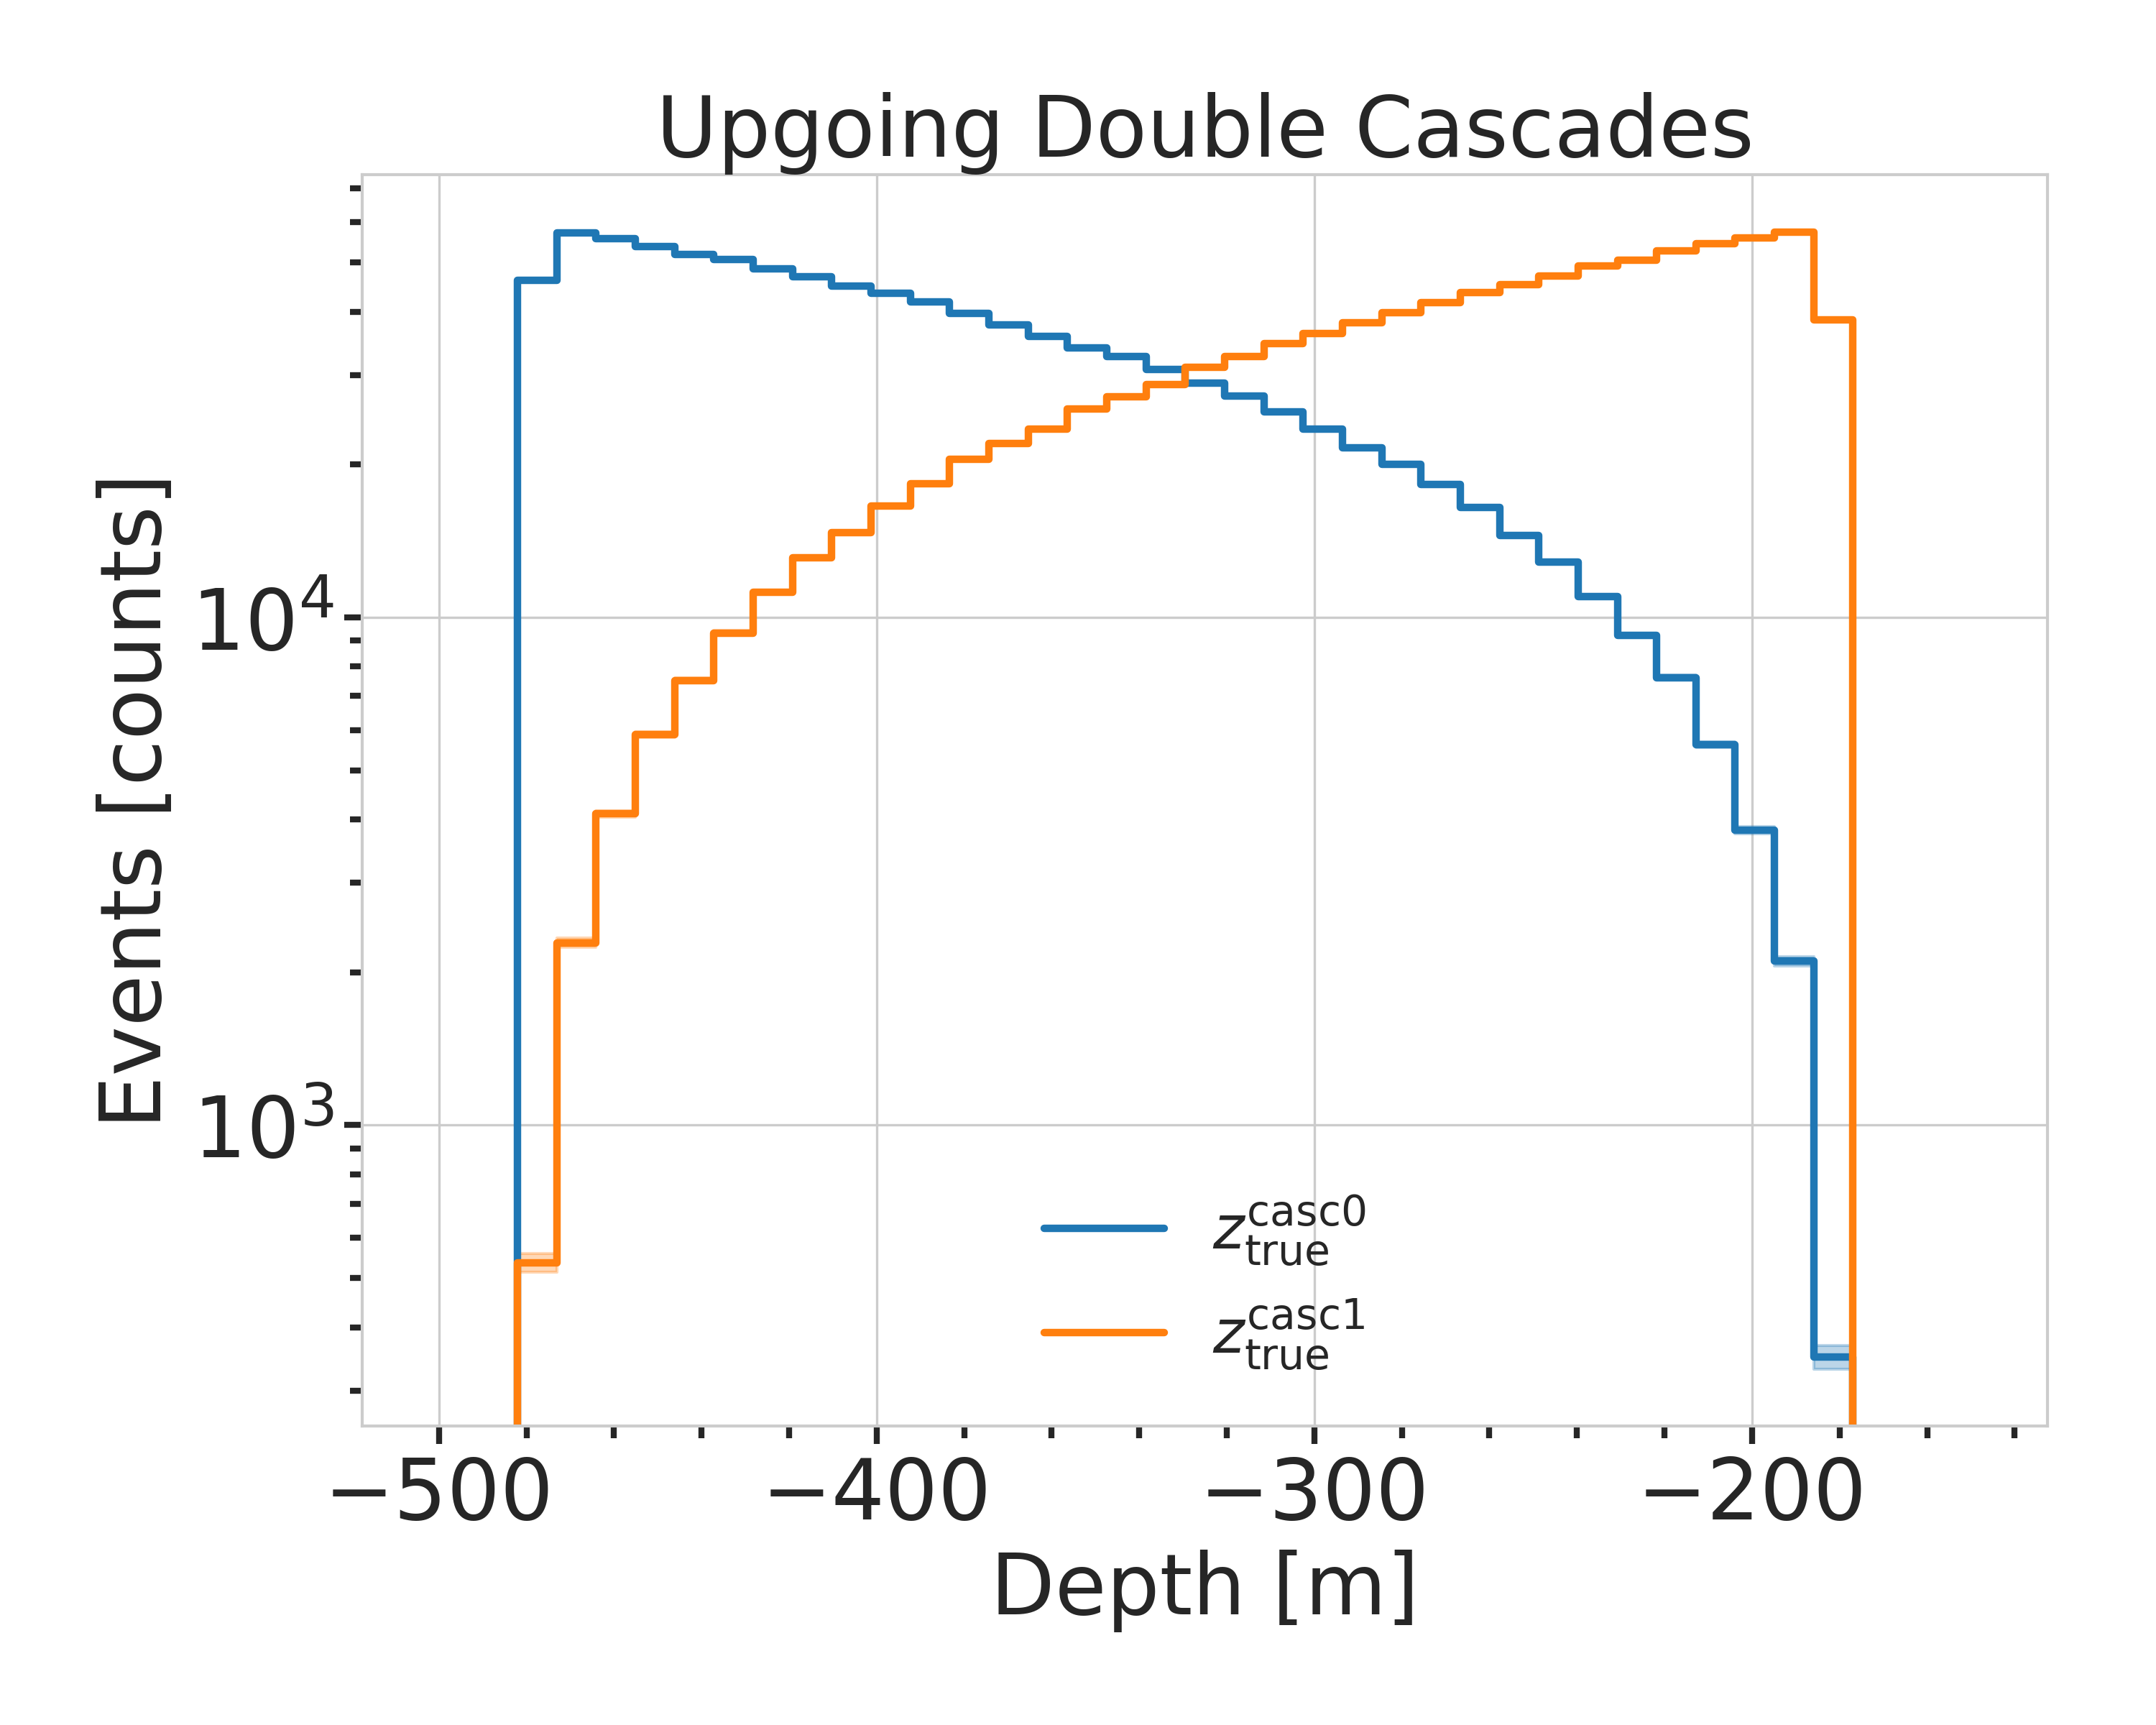
\includegraphics[width=0.49\linewidth]{figures/model_independent_simulation/gen_level/1_d_distr_depths_clipped.png}
    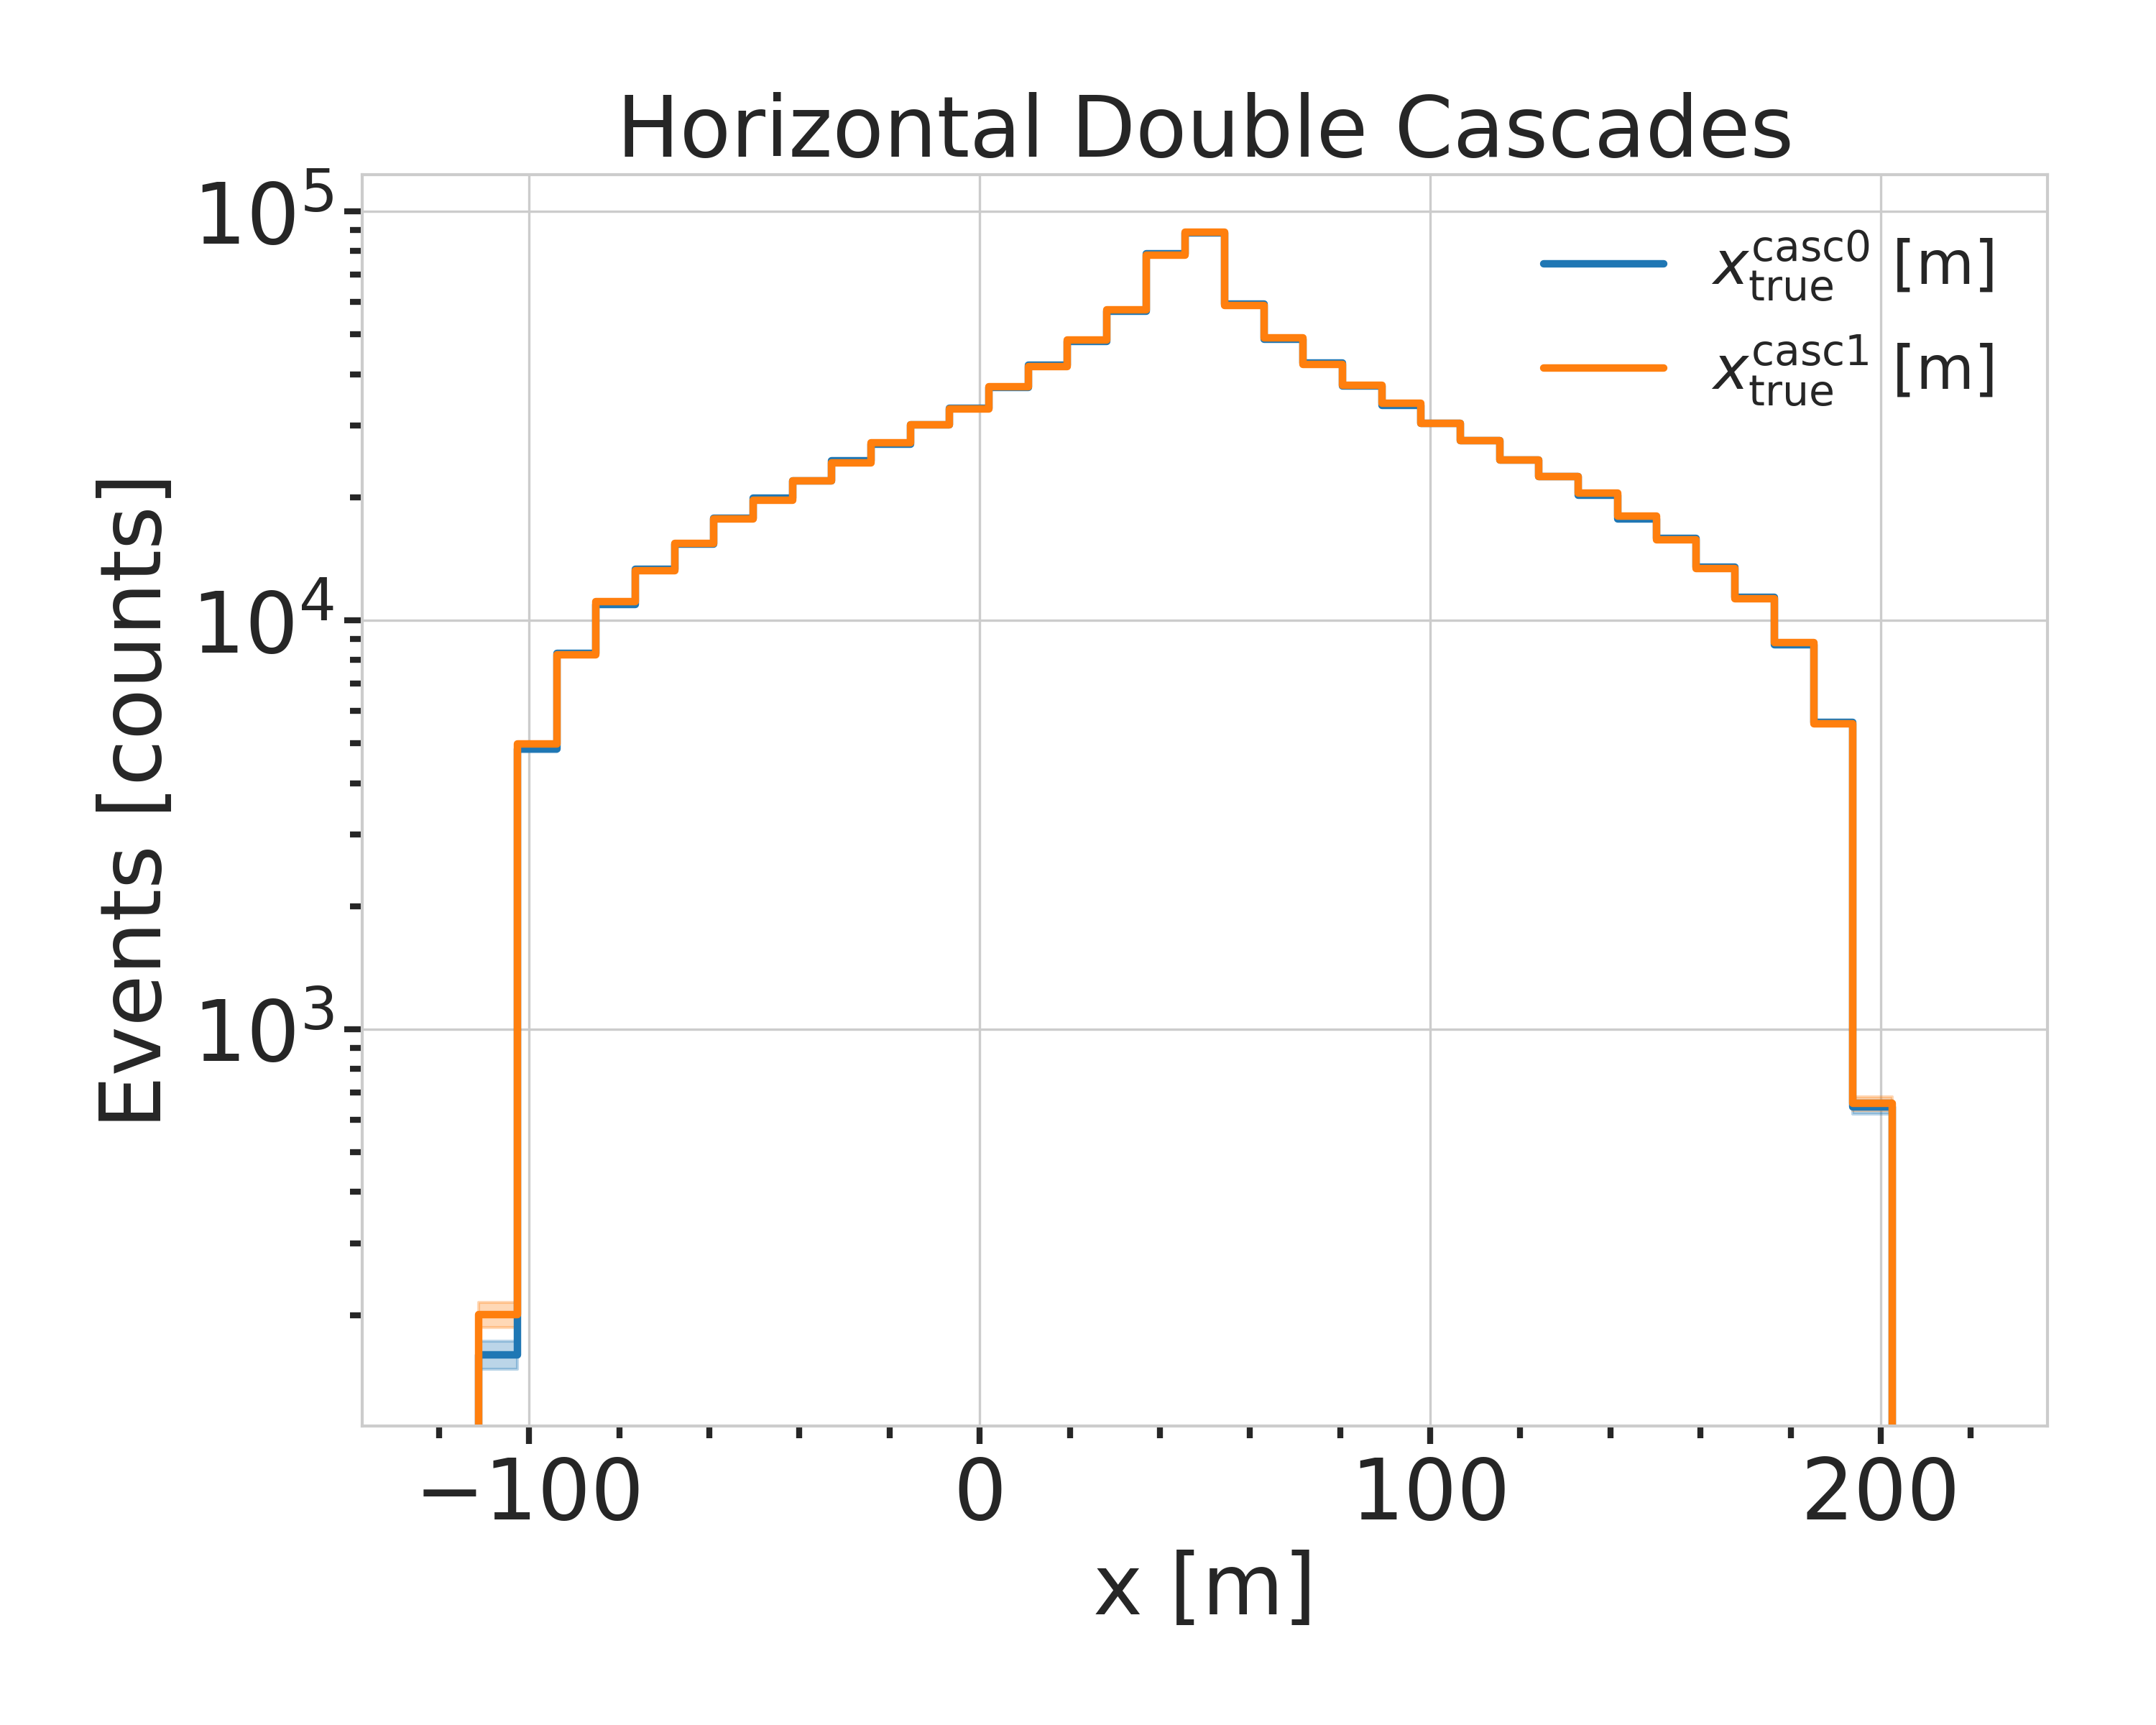
\includegraphics[width=0.49\linewidth]{figures/model_independent_simulation/gen_level/1_d_distr_xs_clipped.png}
    \caption[Simplified model independent simulation generation level distributions]{Generation level distributions of the simplistic simulation sets. Vertical positions (left) and horizontal positions (right) of both sets are shown.}
    \labfig{simplified_gen_distris_appendix}
\end{figure*}

\todo{Re-make plot with x,y for horizontal set one plot!}

\begin{figure*}
    \centering
    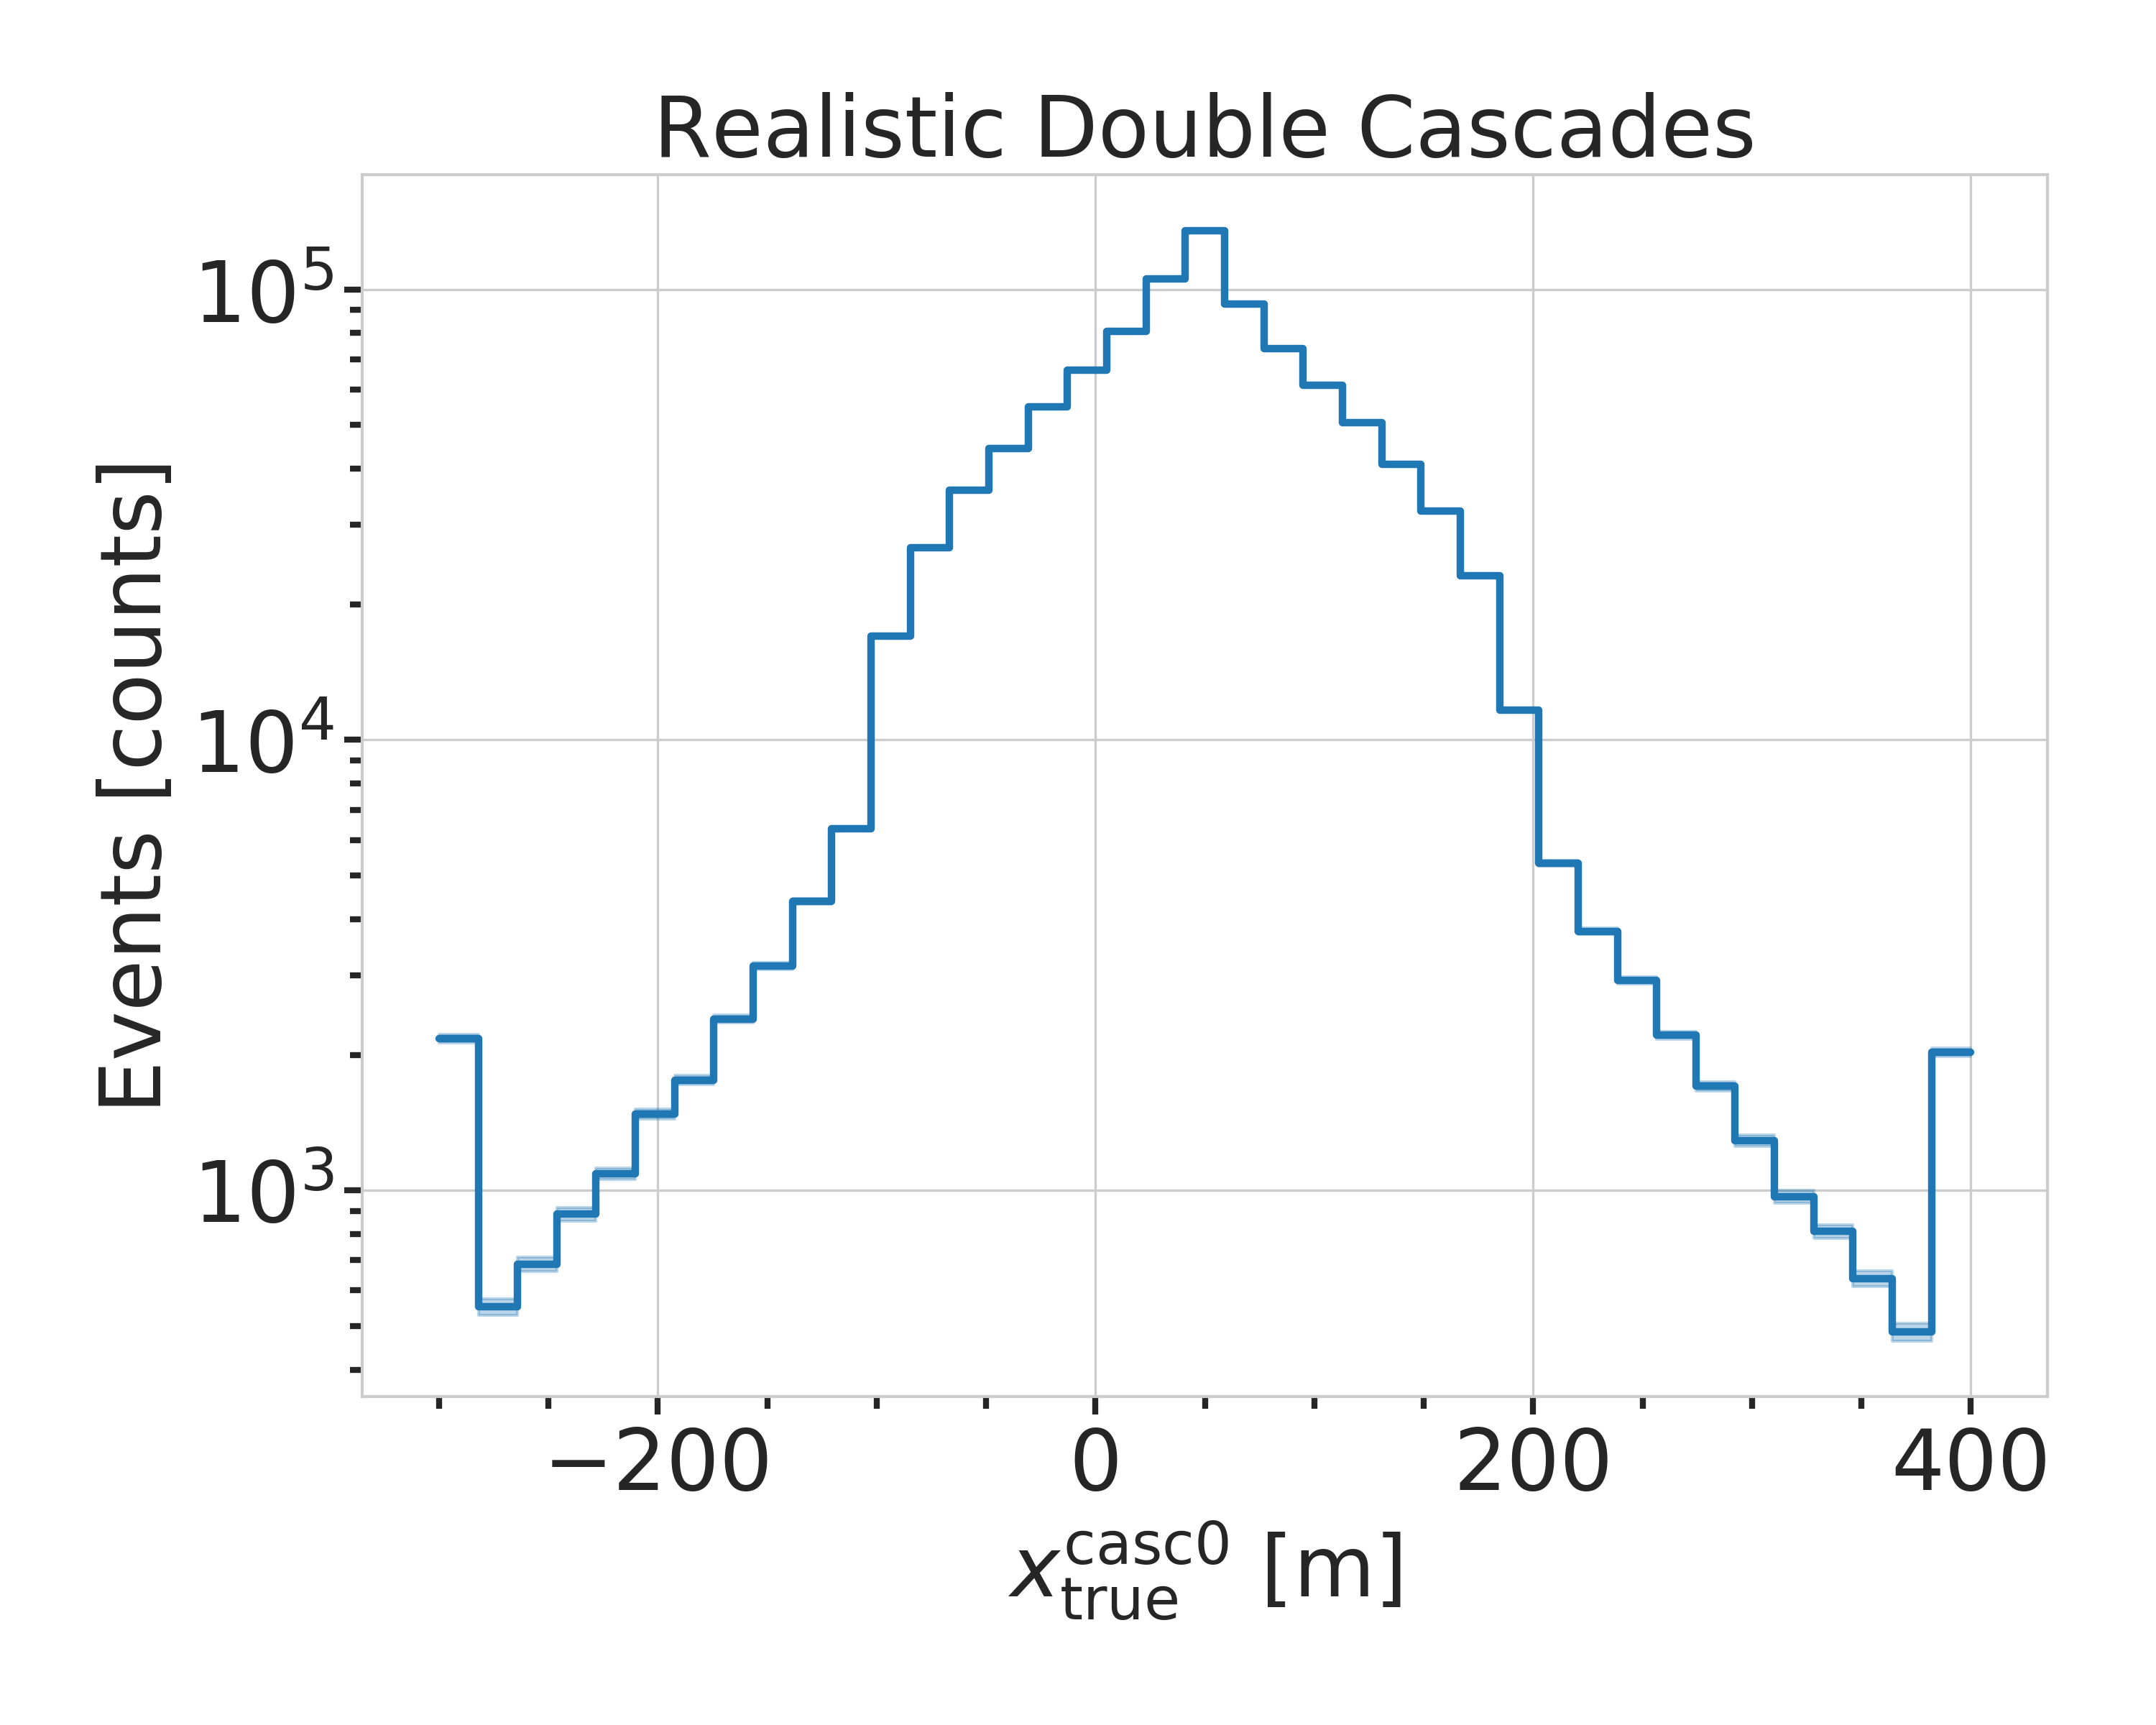
\includegraphics[width=0.49\linewidth]{figures/model_independent_simulation/gen_level/194603_gen_level_1_d_distr_casc0_true_x_clipped.png}
    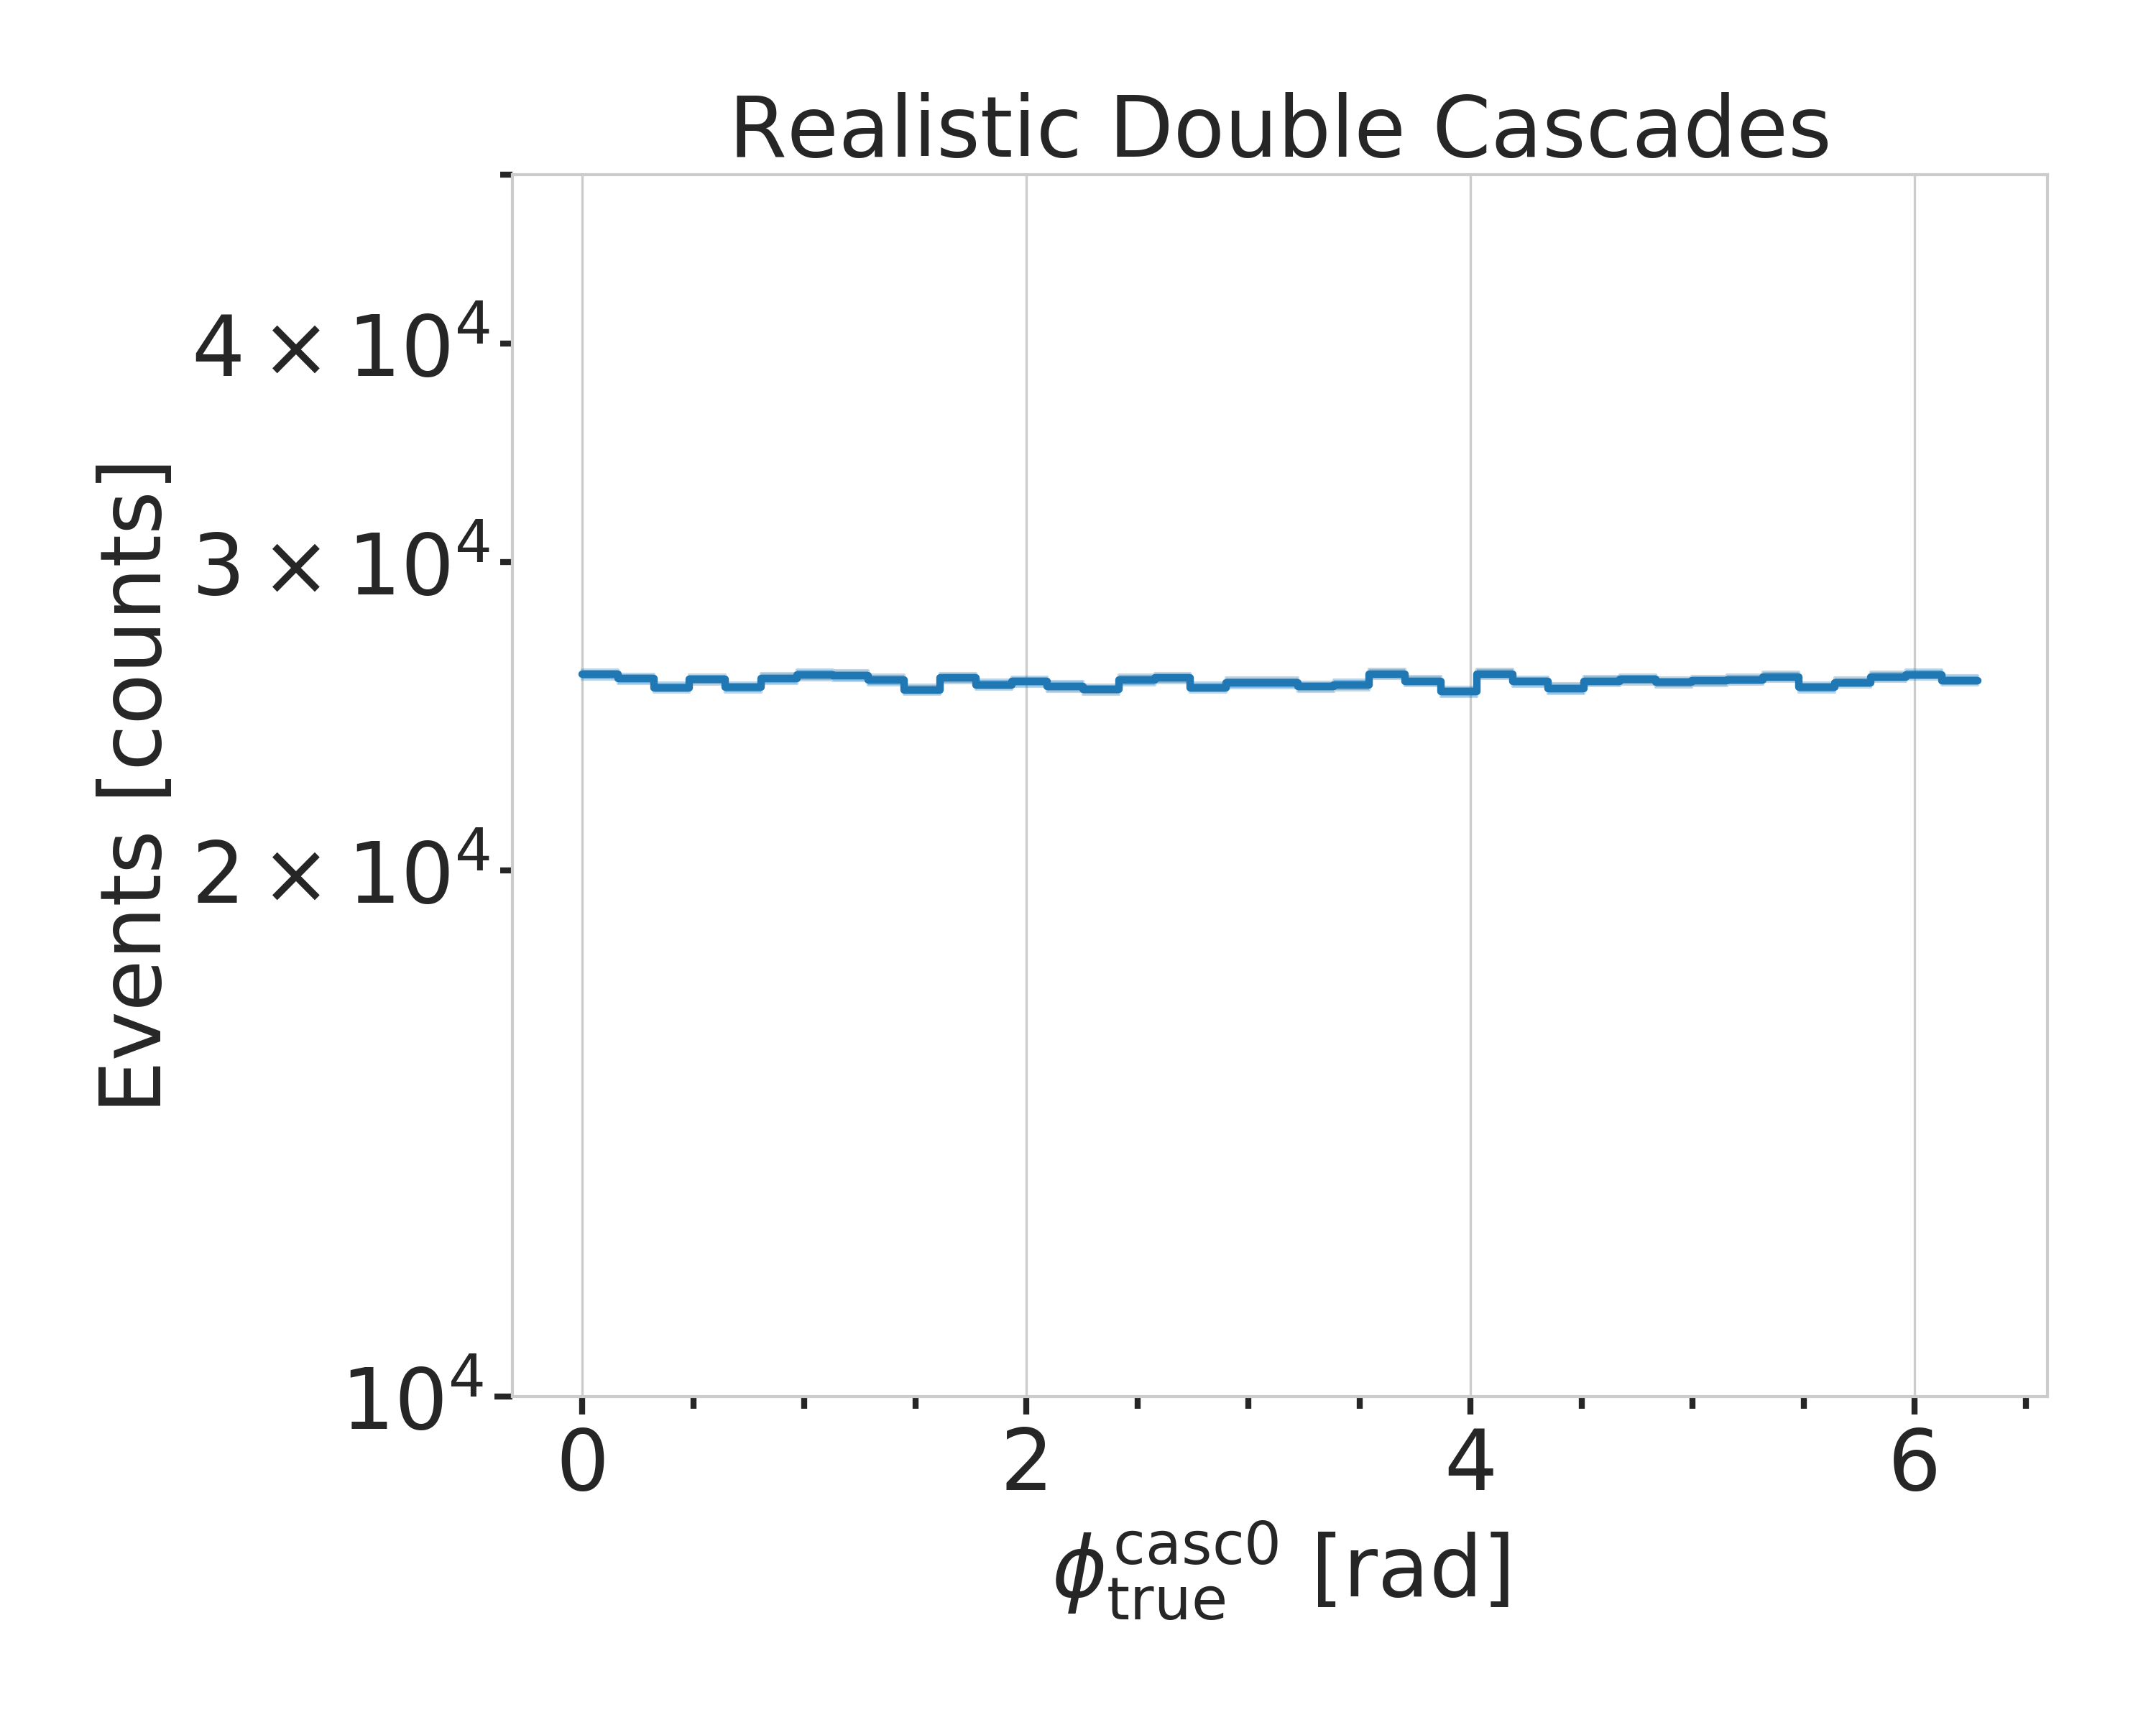
\includegraphics[width=0.49\linewidth]{figures/model_independent_simulation/gen_level/194603_gen_level_1_d_distr_casc0_true_azimuth_clipped.png}
    \caption[Realistic model independent simulation generation level distributions]{Generation level distributions of the realistic simulation set. Shown are the cascade $x, y, z$ positions (left) and direction angles (right).}
    \labfig{realistic_gen_distris_appendix}
\end{figure*}

\todo{Re-make plot with x, y, z for both cascades in one.}
\todo{Re-arrange plots in a more sensible way.}


\section{Model Dependent Simulation Distributions} \labsec{model_dependent_simulation_appendix}

\begin{figure*}[h]
    \centering
    \begin{subfigure}{0.49\linewidth}
        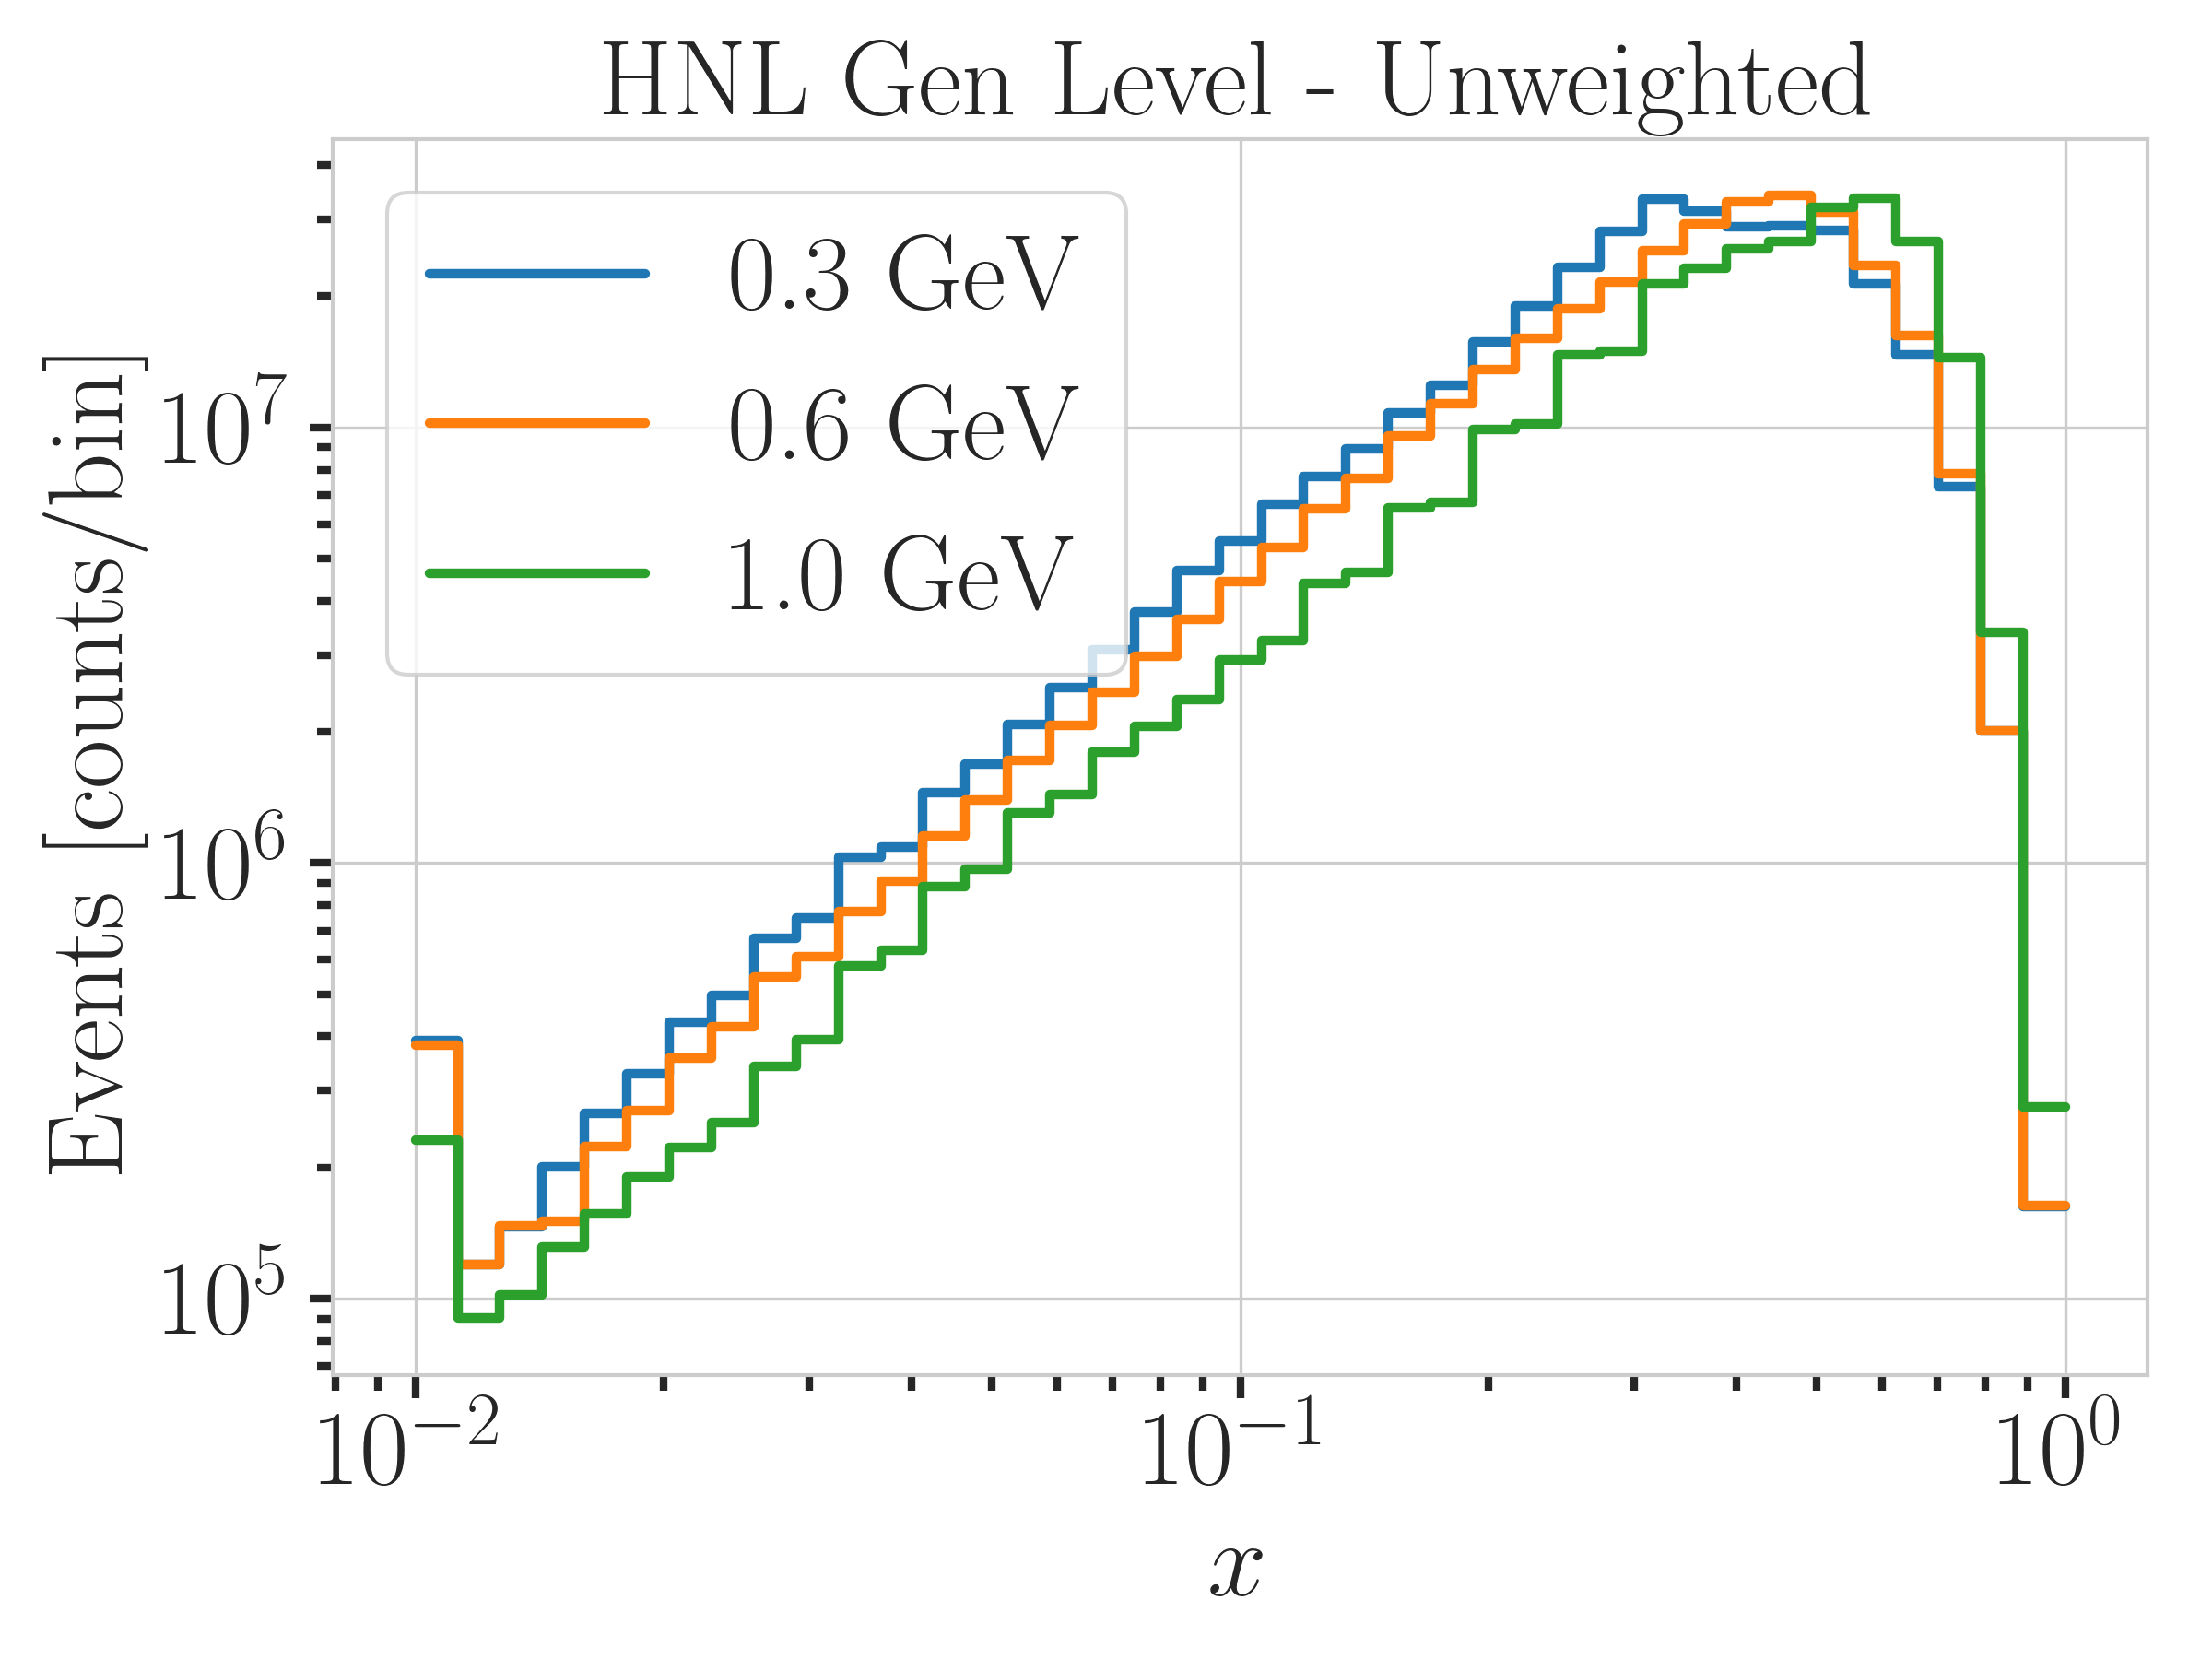
\includegraphics{figures/hnl_simulation/generation/1_d_distr_finalStateX_gen_level_unweighted.png}
        \caption{Bjorken x}
    \end{subfigure}
    \begin{subfigure}{0.49\linewidth}
    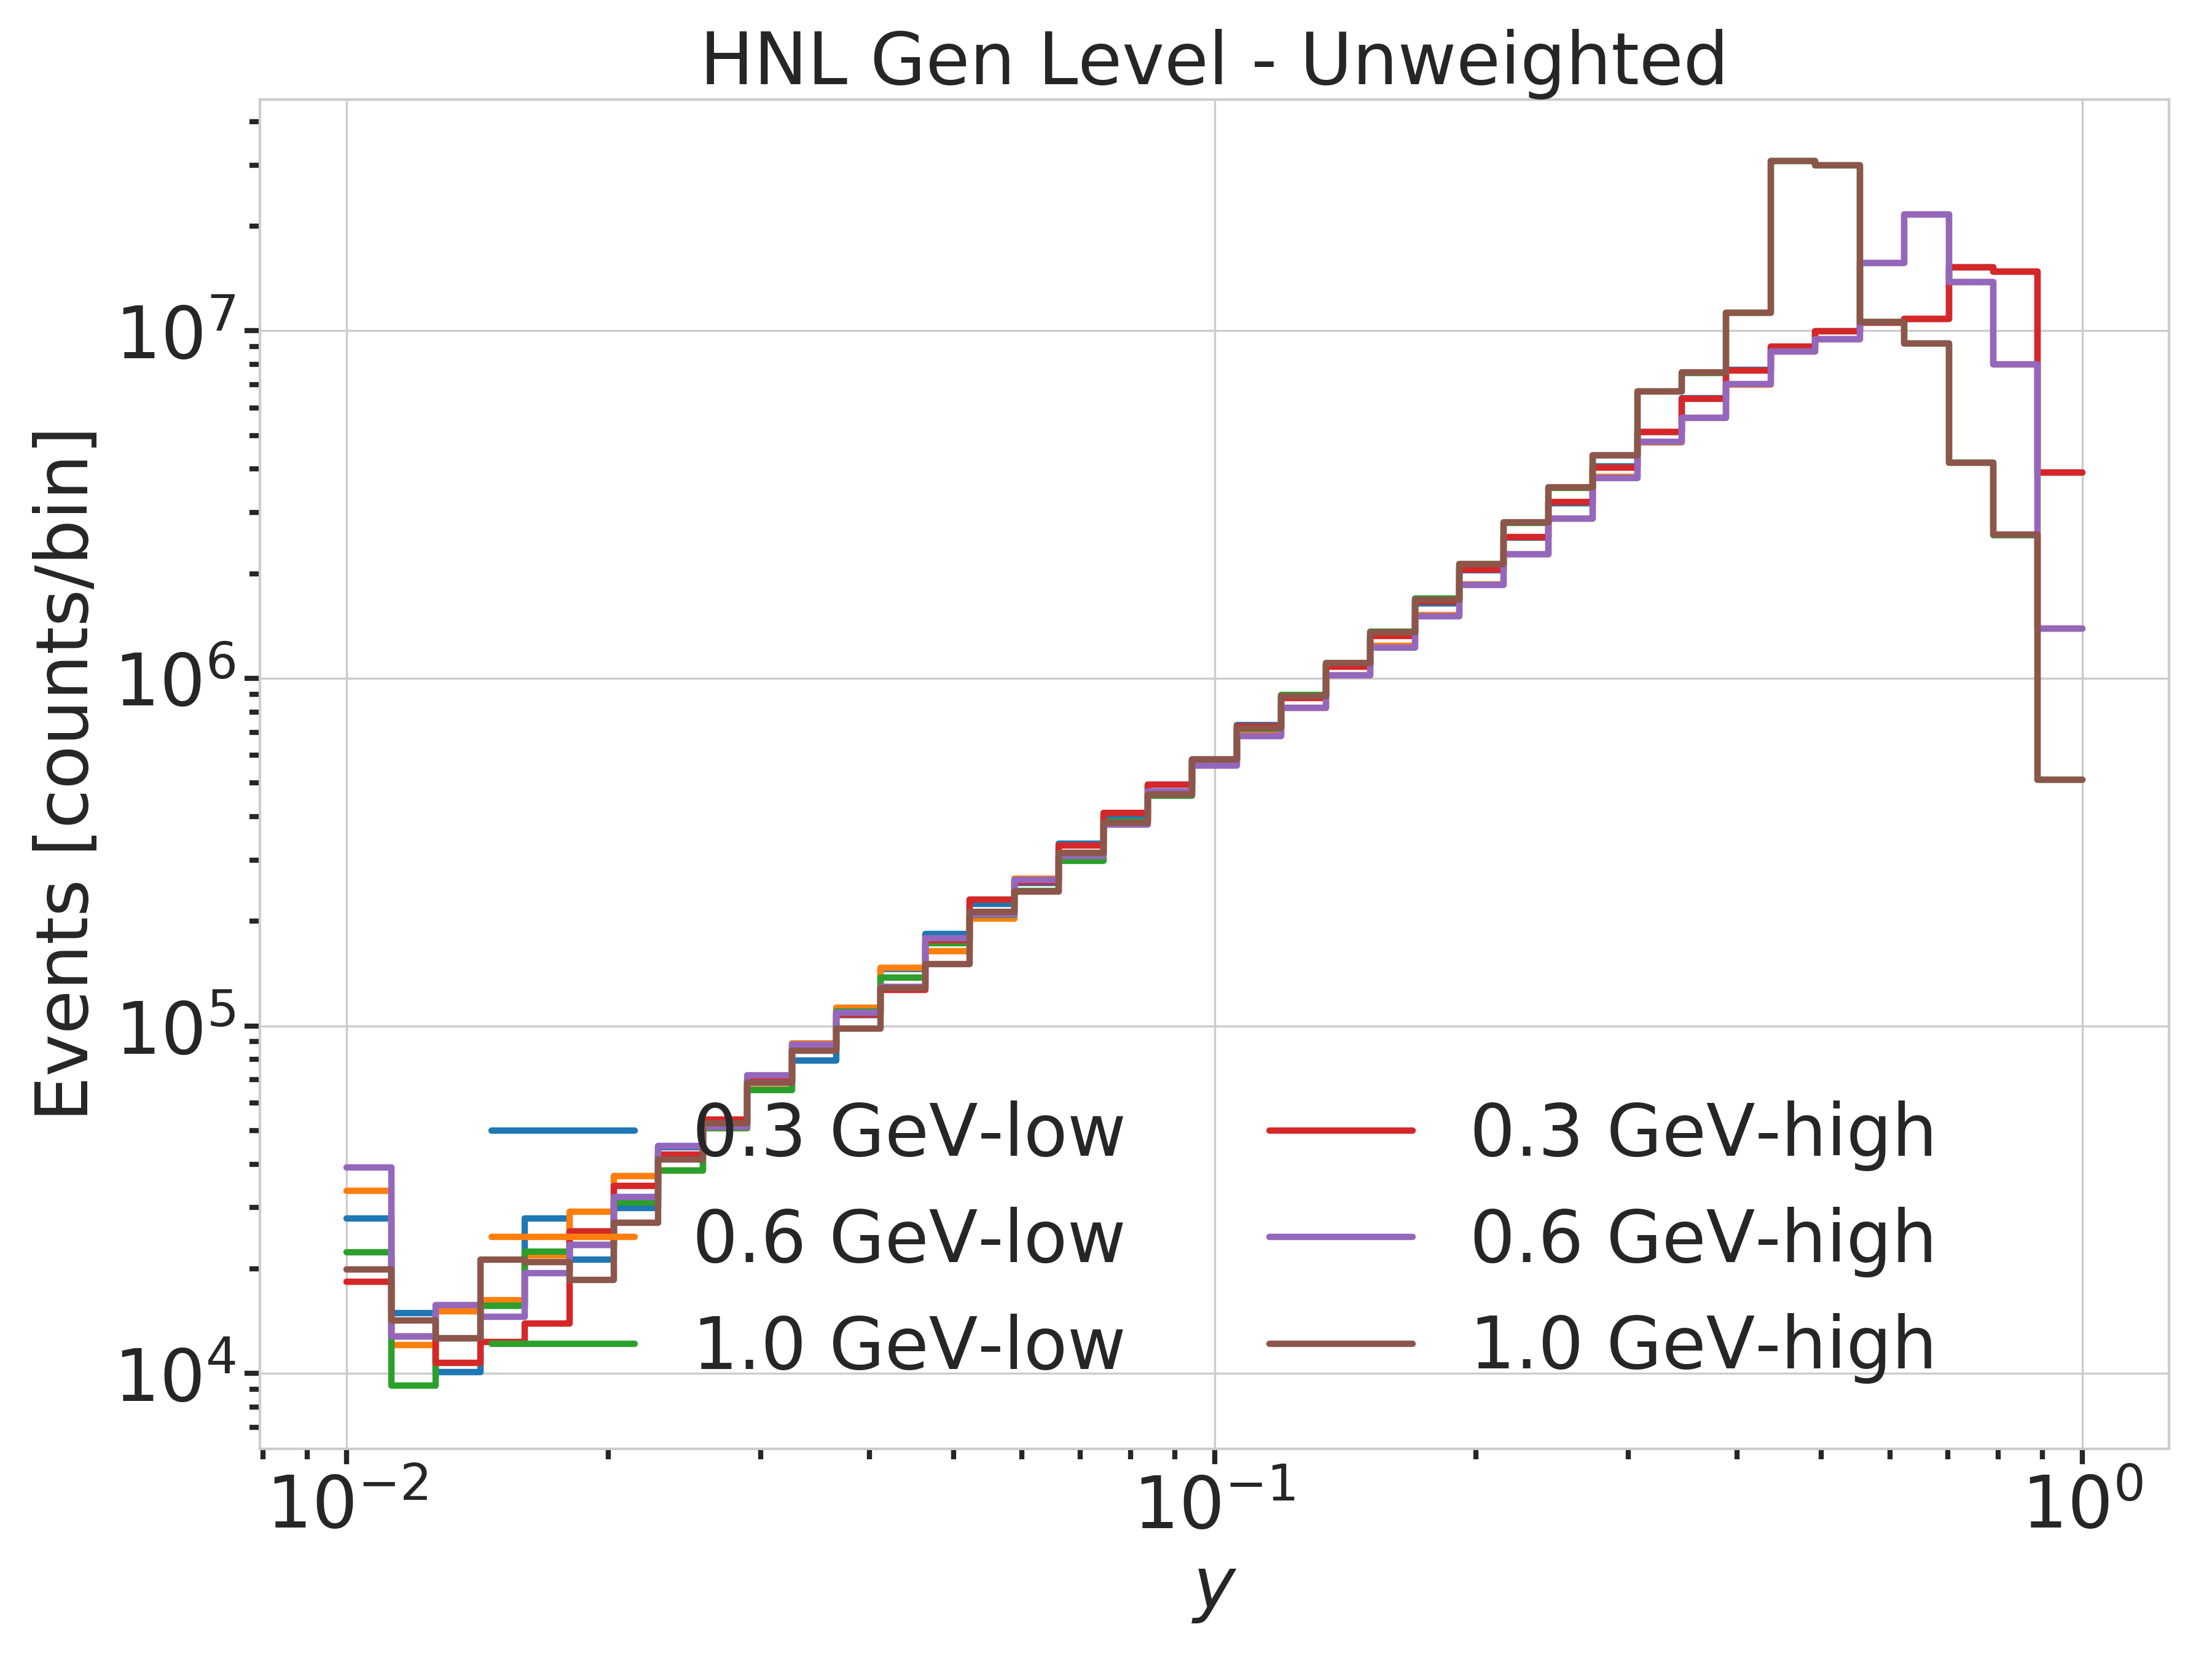
\includegraphics{figures/hnl_simulation/generation/1_d_distr_finalStateY_gen_level_unweighted.png}
        \caption{Bjorken y}
    \end{subfigure}
    \caption[Model dependent simulation generation level distributions]{Generation level distributions of the model dependent simulation.}
    \labfig{hnl_gen_distris_appendix}
\end{figure*}


\setchapterstyle{lines}
\chapter{Analysis Checks}
\labch{analysis_checks}


\section{Minimization Robustness} \labsec{asimov_inject_recover_appendix}

\reffig{asimov_inject_recover_appendix} shows additional Asimov inject/recover tests for the \SI{0.3}{\gev} and the \SI{1.0}{\gev} mass sets. The tests were described in \refsec{asimov_inject_recover}.

\begin{figure*}[h]
    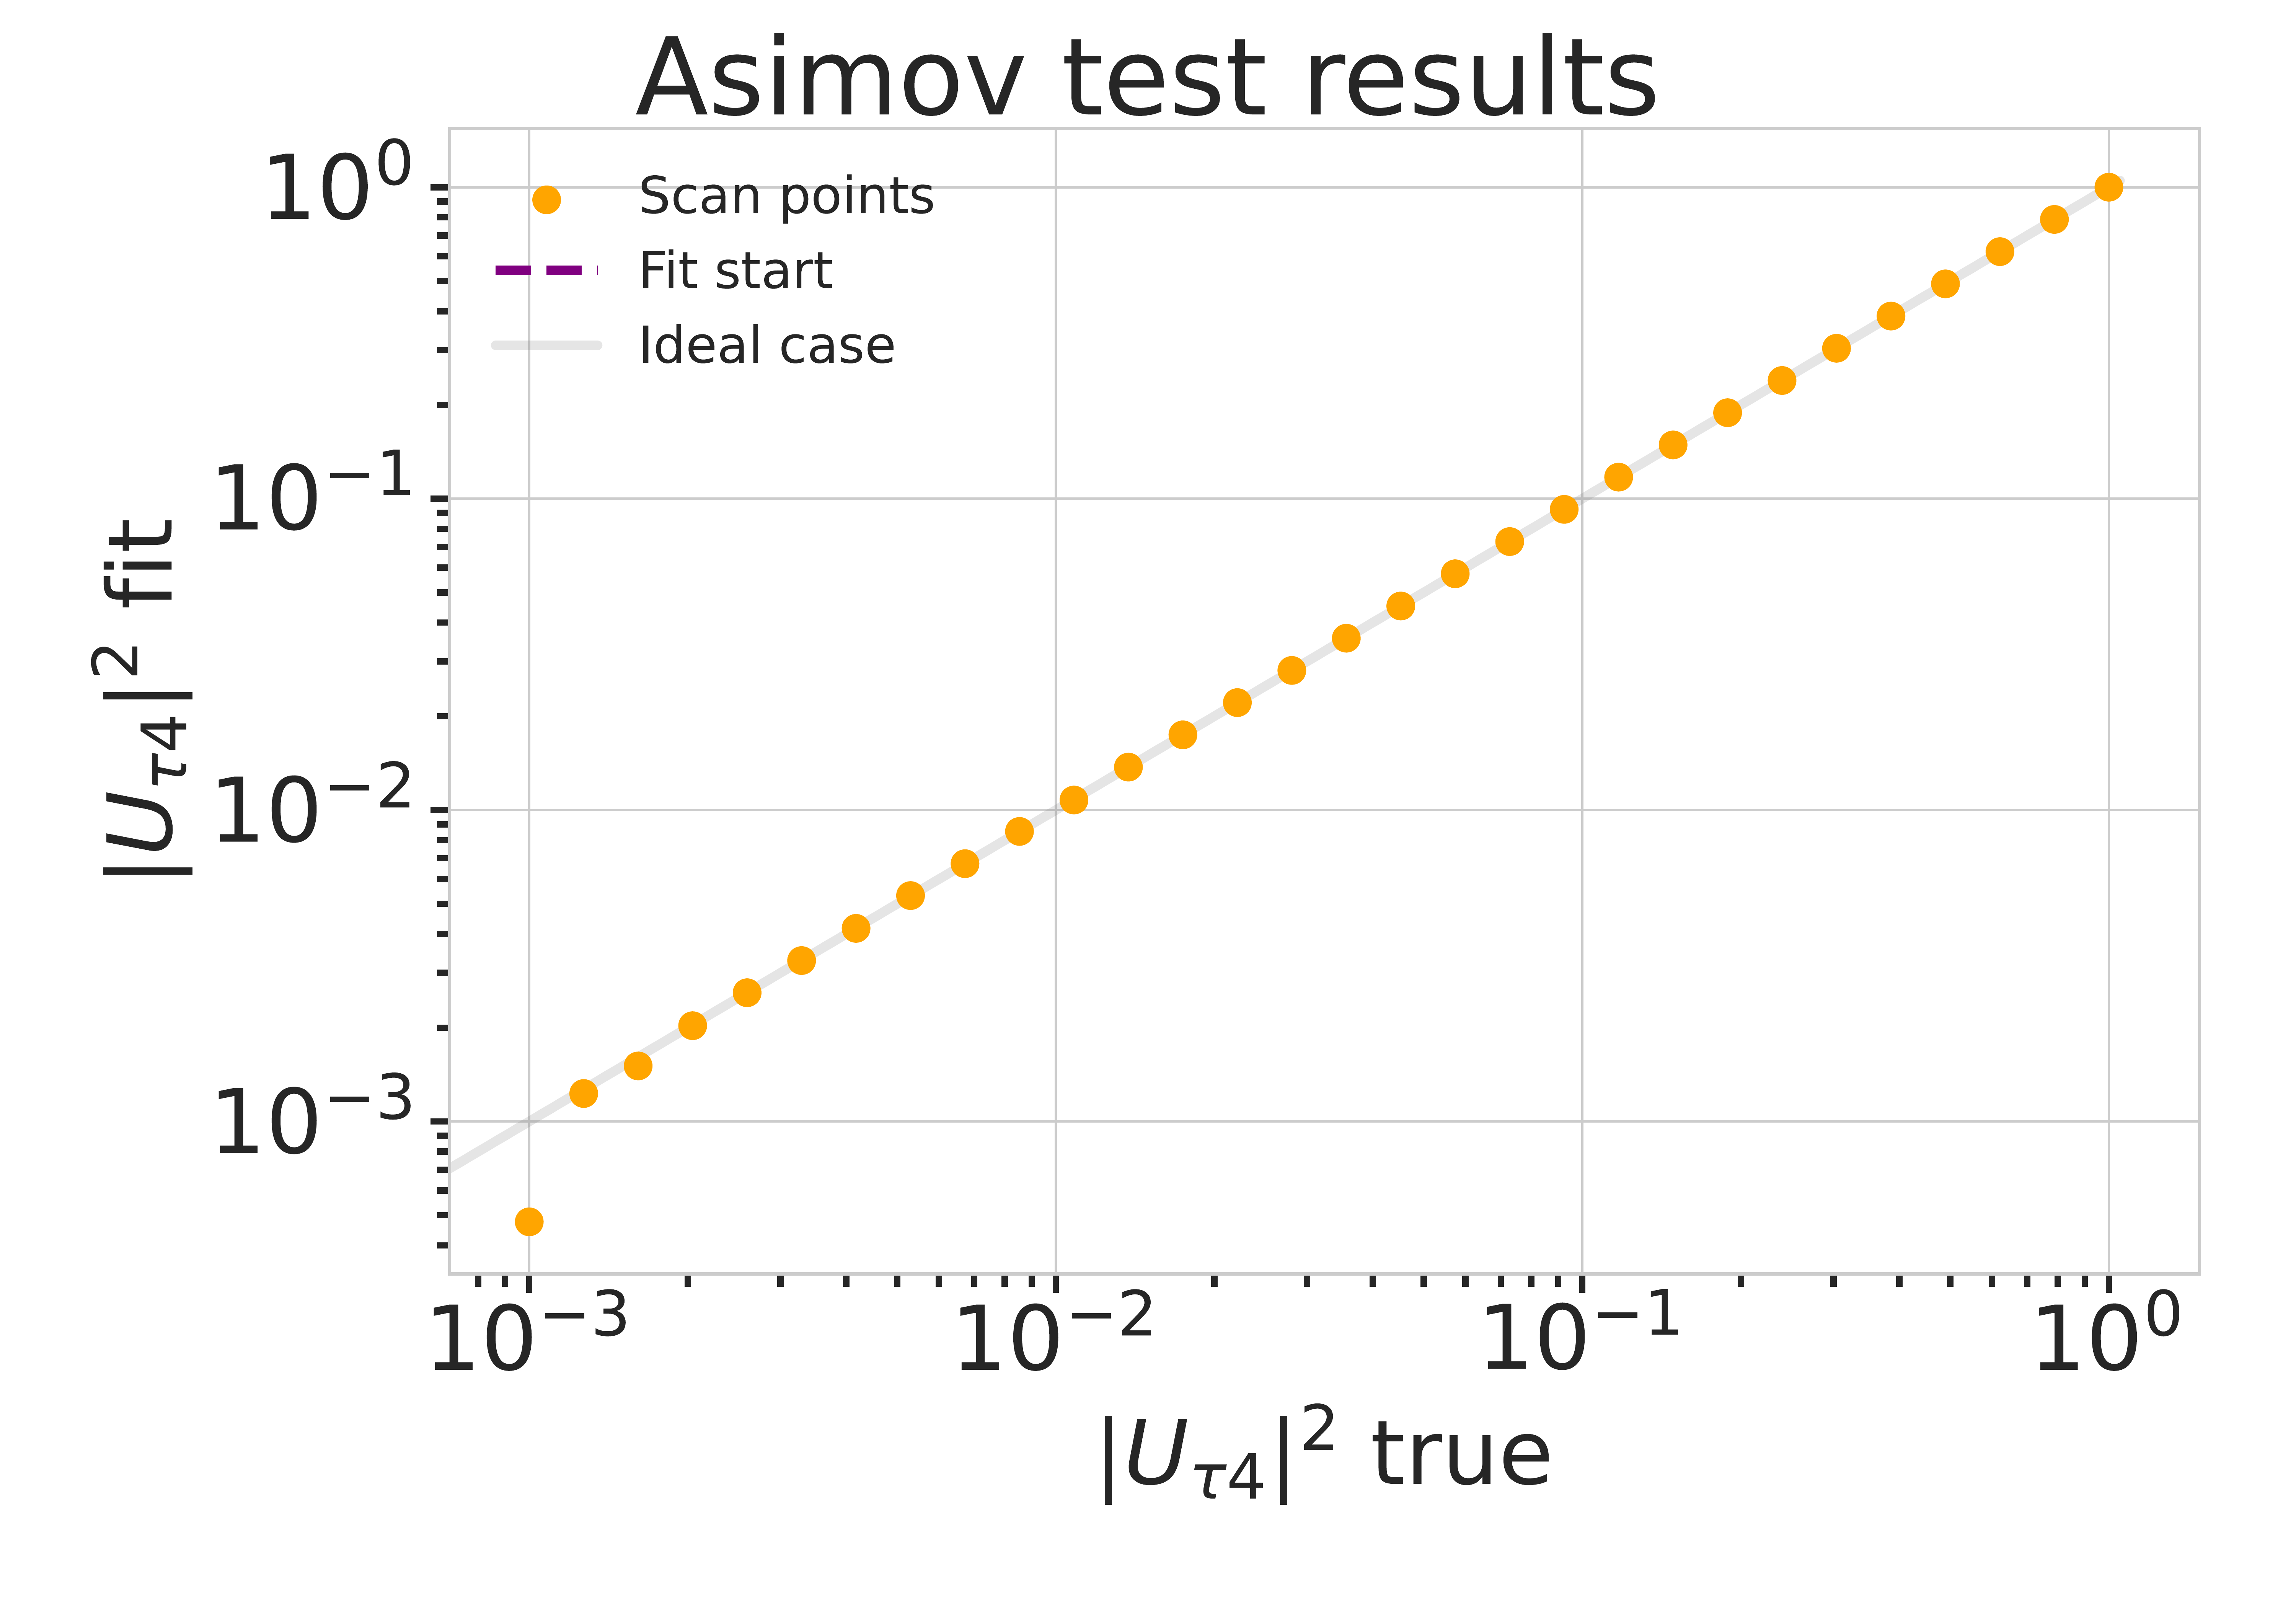
\includegraphics[width=0.49\linewidth]{figures/results/checks/asimov_scan_0.3_GeV-01.png}
    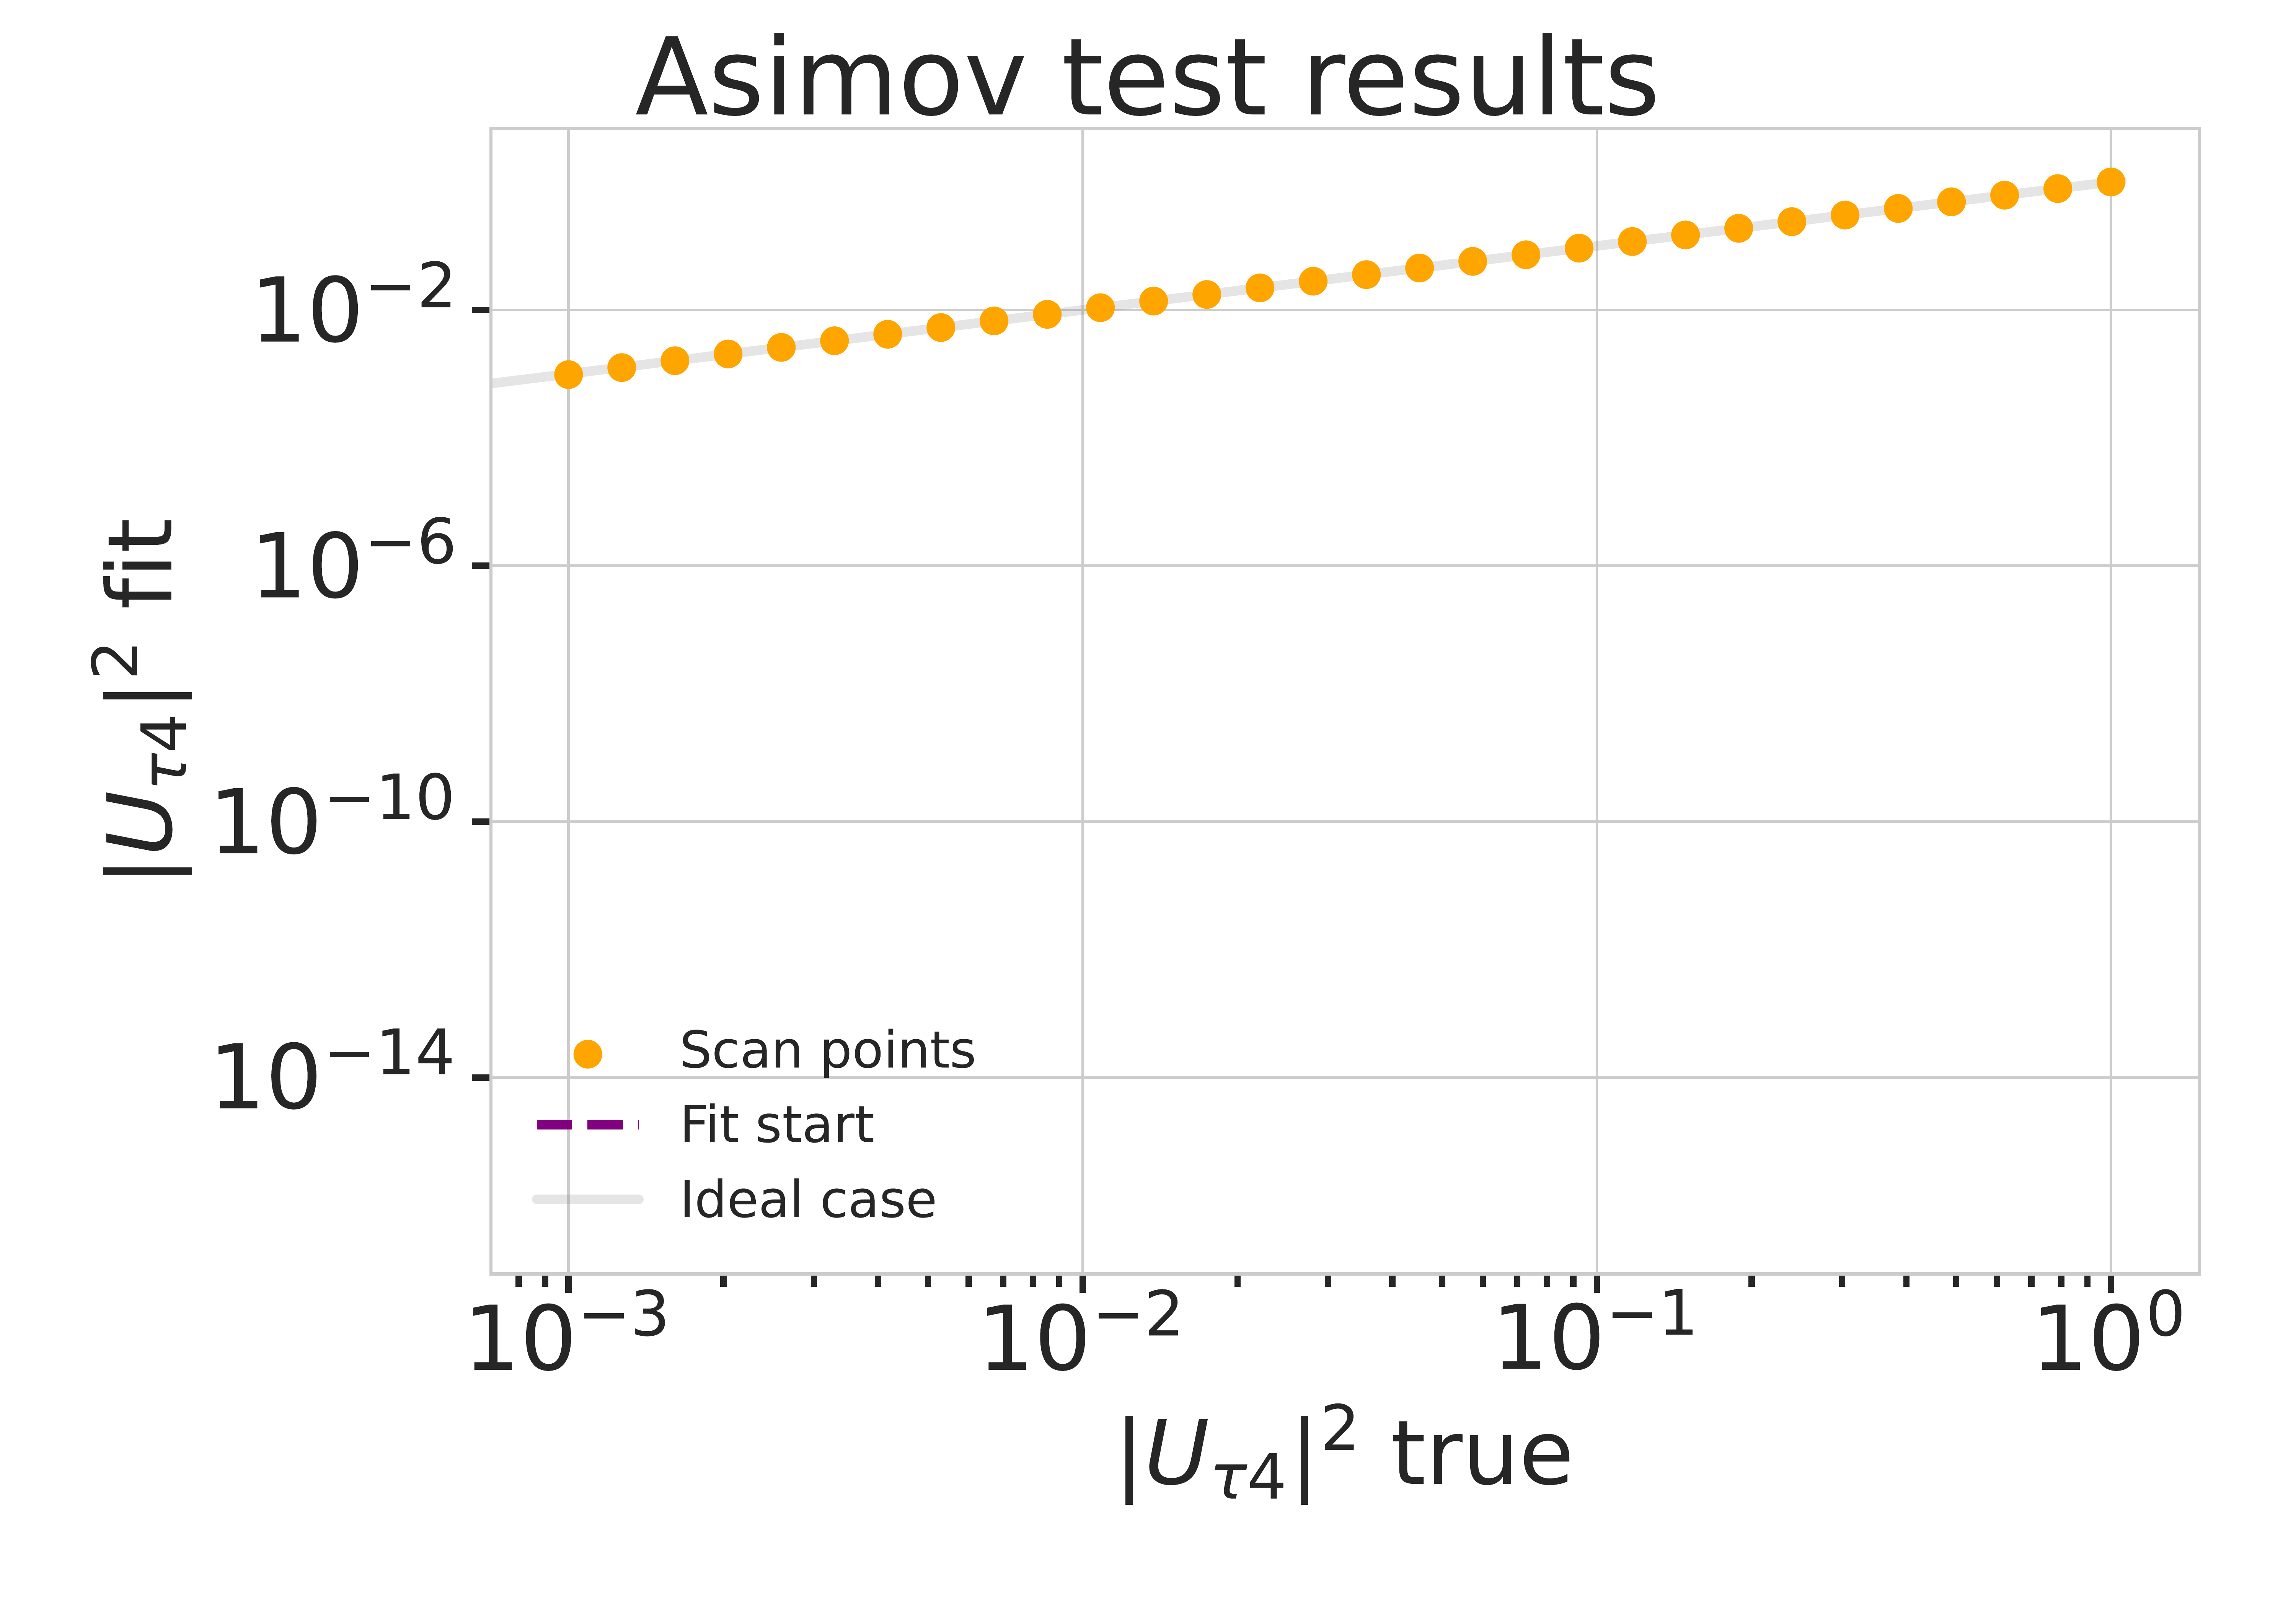
\includegraphics[width=0.49\linewidth]{figures/results/checks/asimov_scan_1.0_GeV-01.png}
	\caption[Asimov inject/recover test (\SI{0.3}{\gev}, \SI{1.0}{\gev})]{Asimov inject/recover test for the \SI{0.3}{\gev} (left) and the \SI{1.0}{\gev} (right) mass sets. Mixing values between $10^{-3}$ and $10^{0}$ are injected and fit back with the full analysis chain. The injected parameter is always recovered within the statistical uncertainty.}
    \labfig{asimov_inject_recover_appendix}
\end{figure*}


% \section{Sensitivities}

% \begin{figure}[h]
%     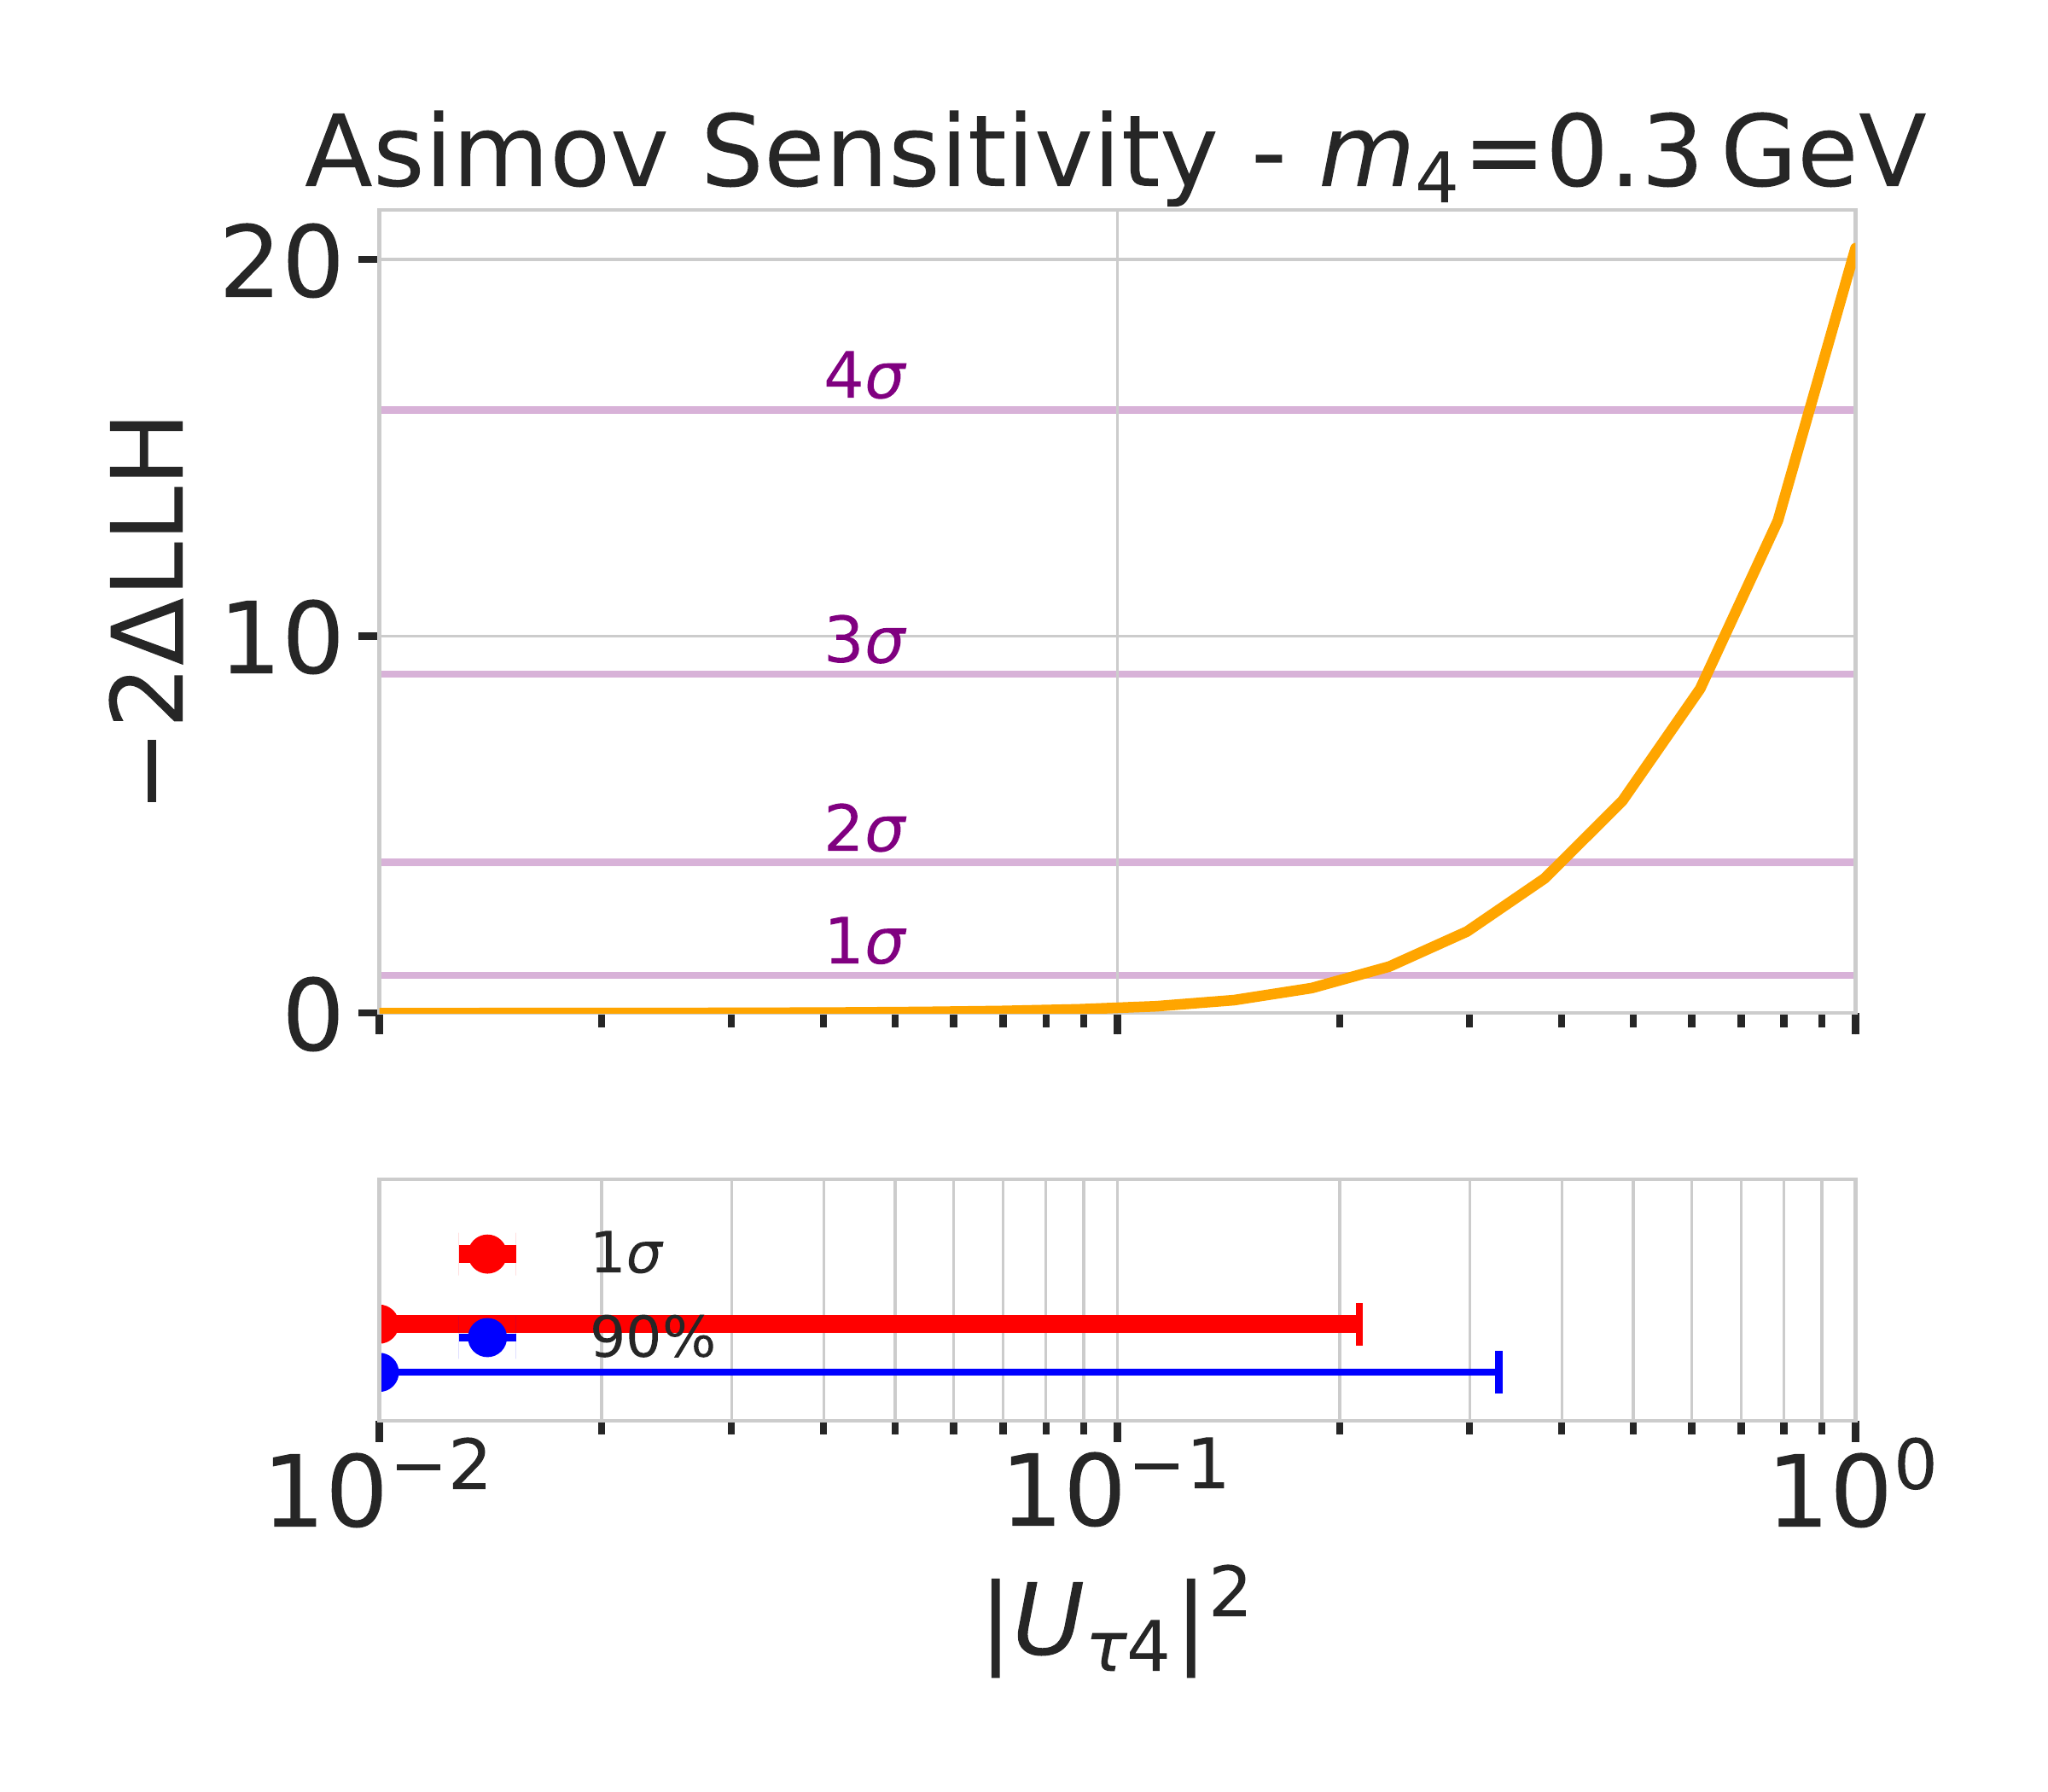
\includegraphics[width=0.49\linewidth]{figures/results/checks/sensitivity_scan_0.3_GeV-1.png}
%     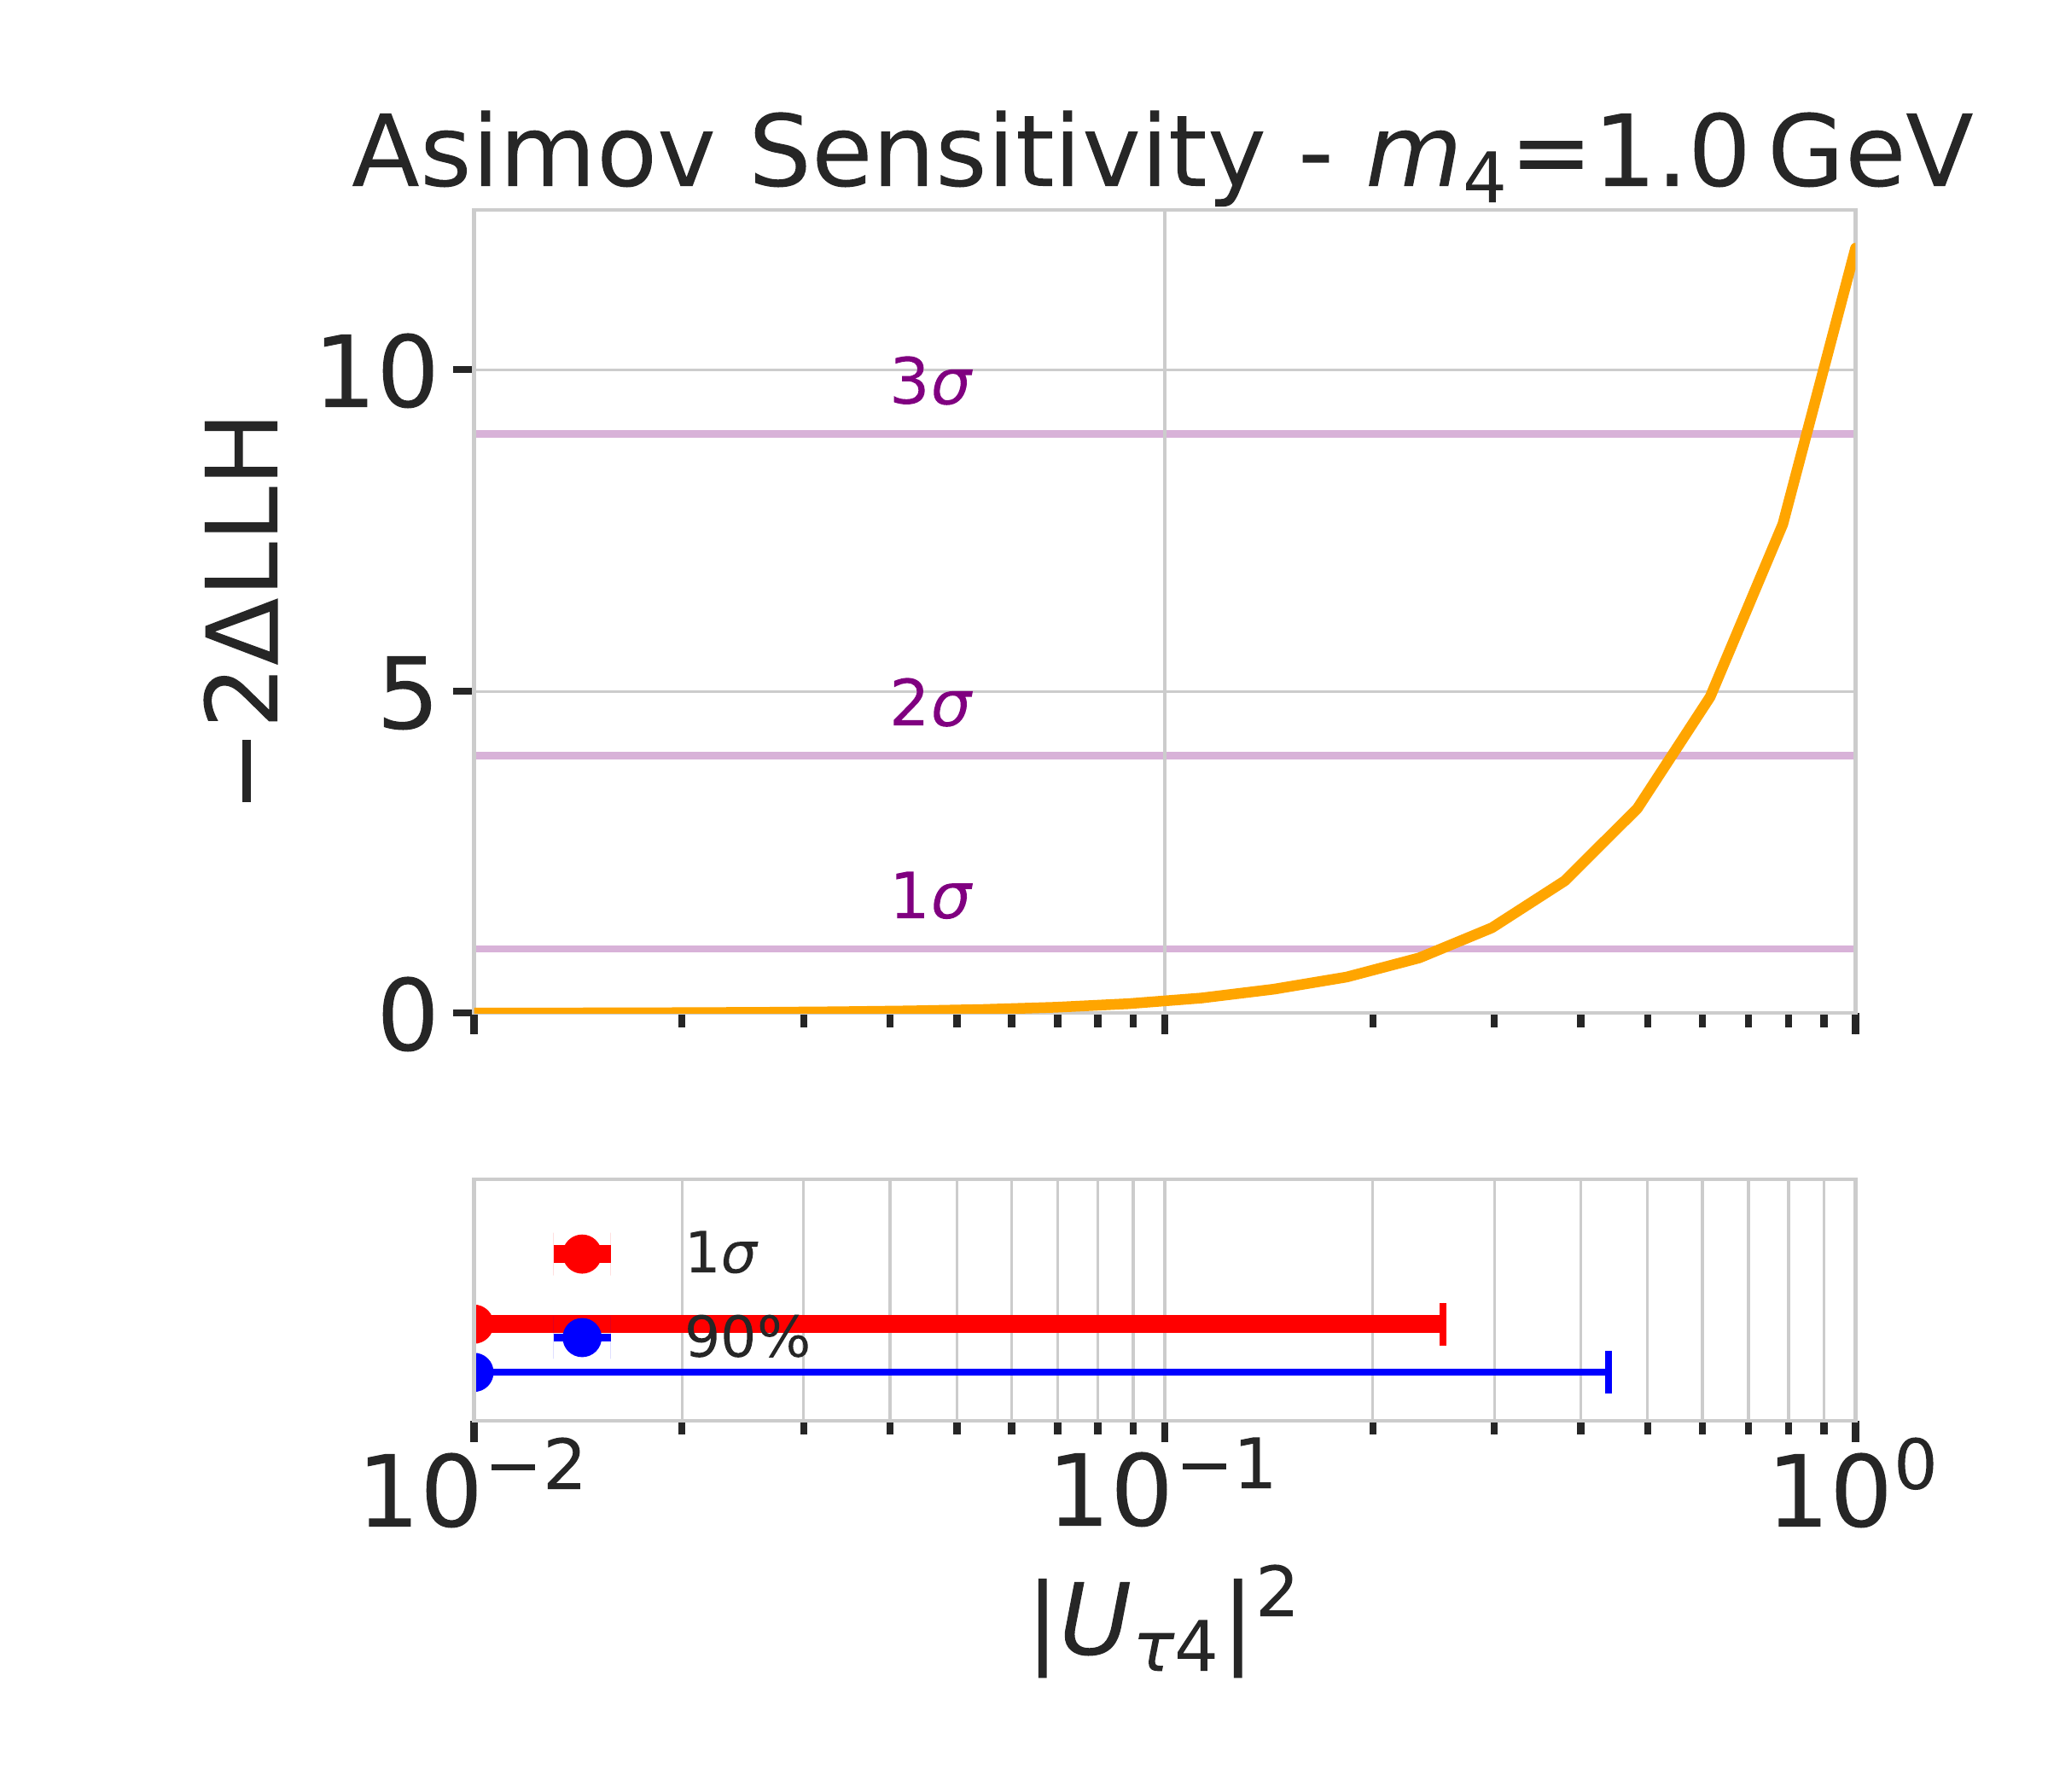
\includegraphics[width=0.49\linewidth]{figures/results/checks/sensitivity_scan_1.0_GeV-1.png}
% 	\caption[Sensitivity scan (\SI{0.3}{\gev}, \SI{1.0}{\gev})]{Sensitivity scan for the \SI{0.3}{\gev} (left) and the \SI{1.0}{\gev} (right) mass sets.}
%     \labfig{sensitivity_scans_appendix}
% \end{figure}


\subsection{Ensemble Tests} \labsec{pseudo_data_ensemble_appendix}

\reffig{pseudo_data_ensemble_appendix} shows additional TS distributions from pseudo-data trials and the observed TS from the fit to the data for the ensemble for the \SI{0.3}{\gev} and the \SI{1.0}{\gev} mass sets. The tests were described in \refsec{pseudo_data_ensemble}.

\begin{figure*}[h]
    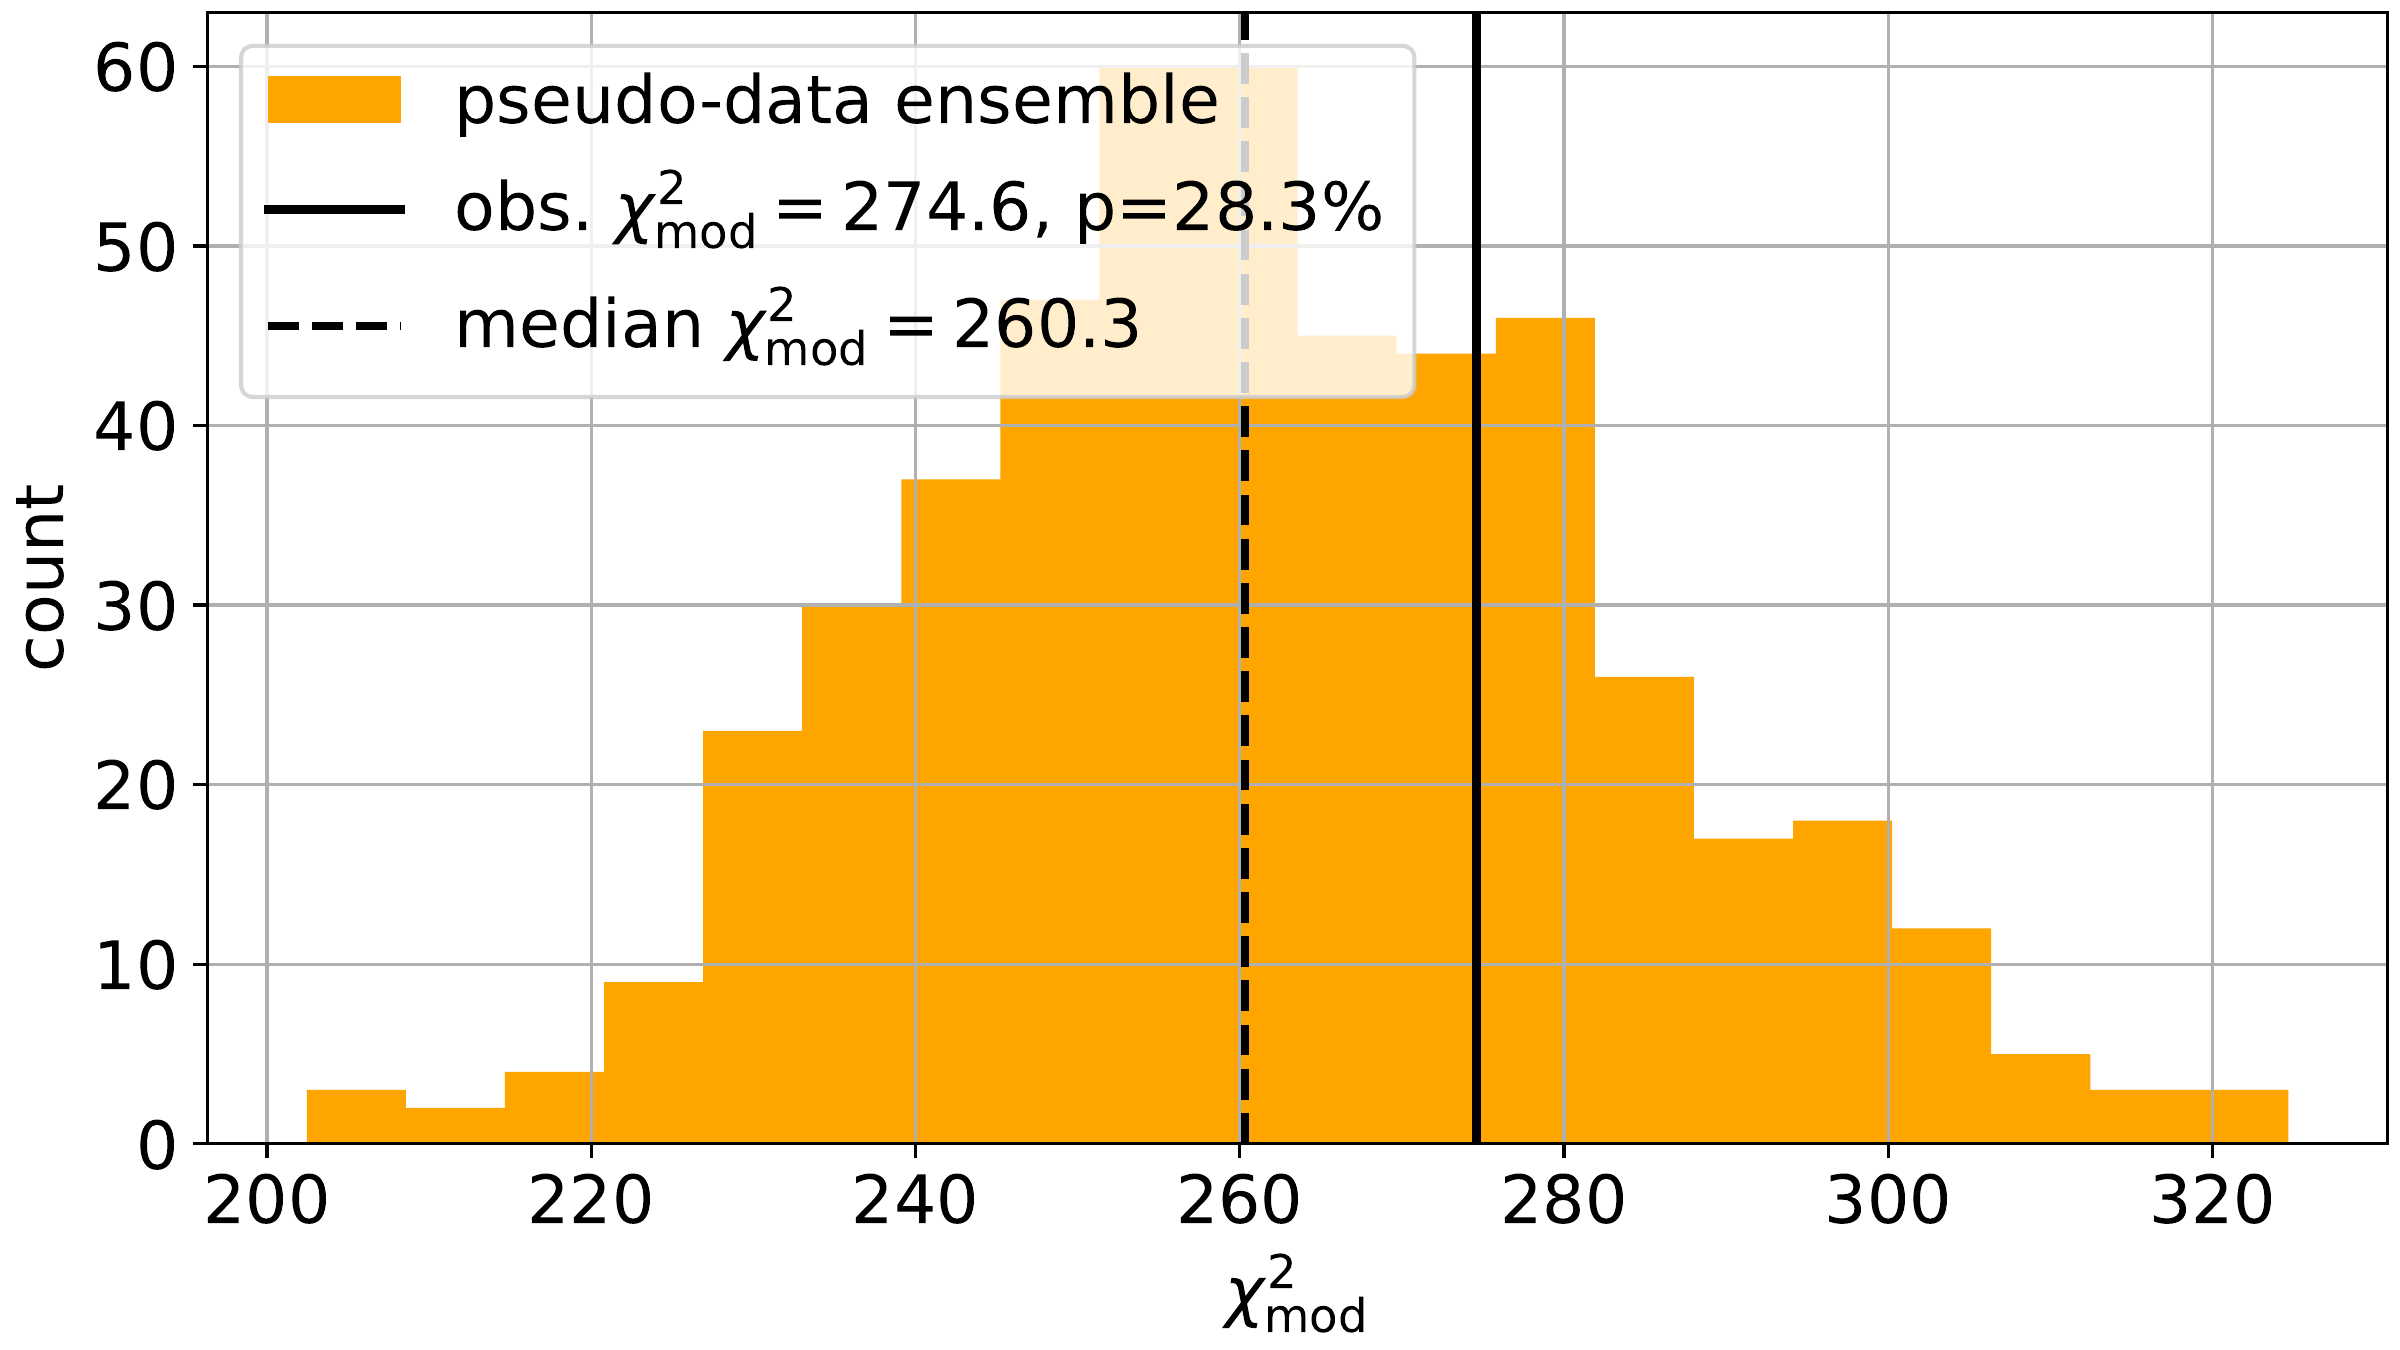
\includegraphics[width=0.49\linewidth]{figures/results/blind_fits/full_blind_fit_0.3_GeV_gauss_plus_poisson_step_3_4-1.png}
    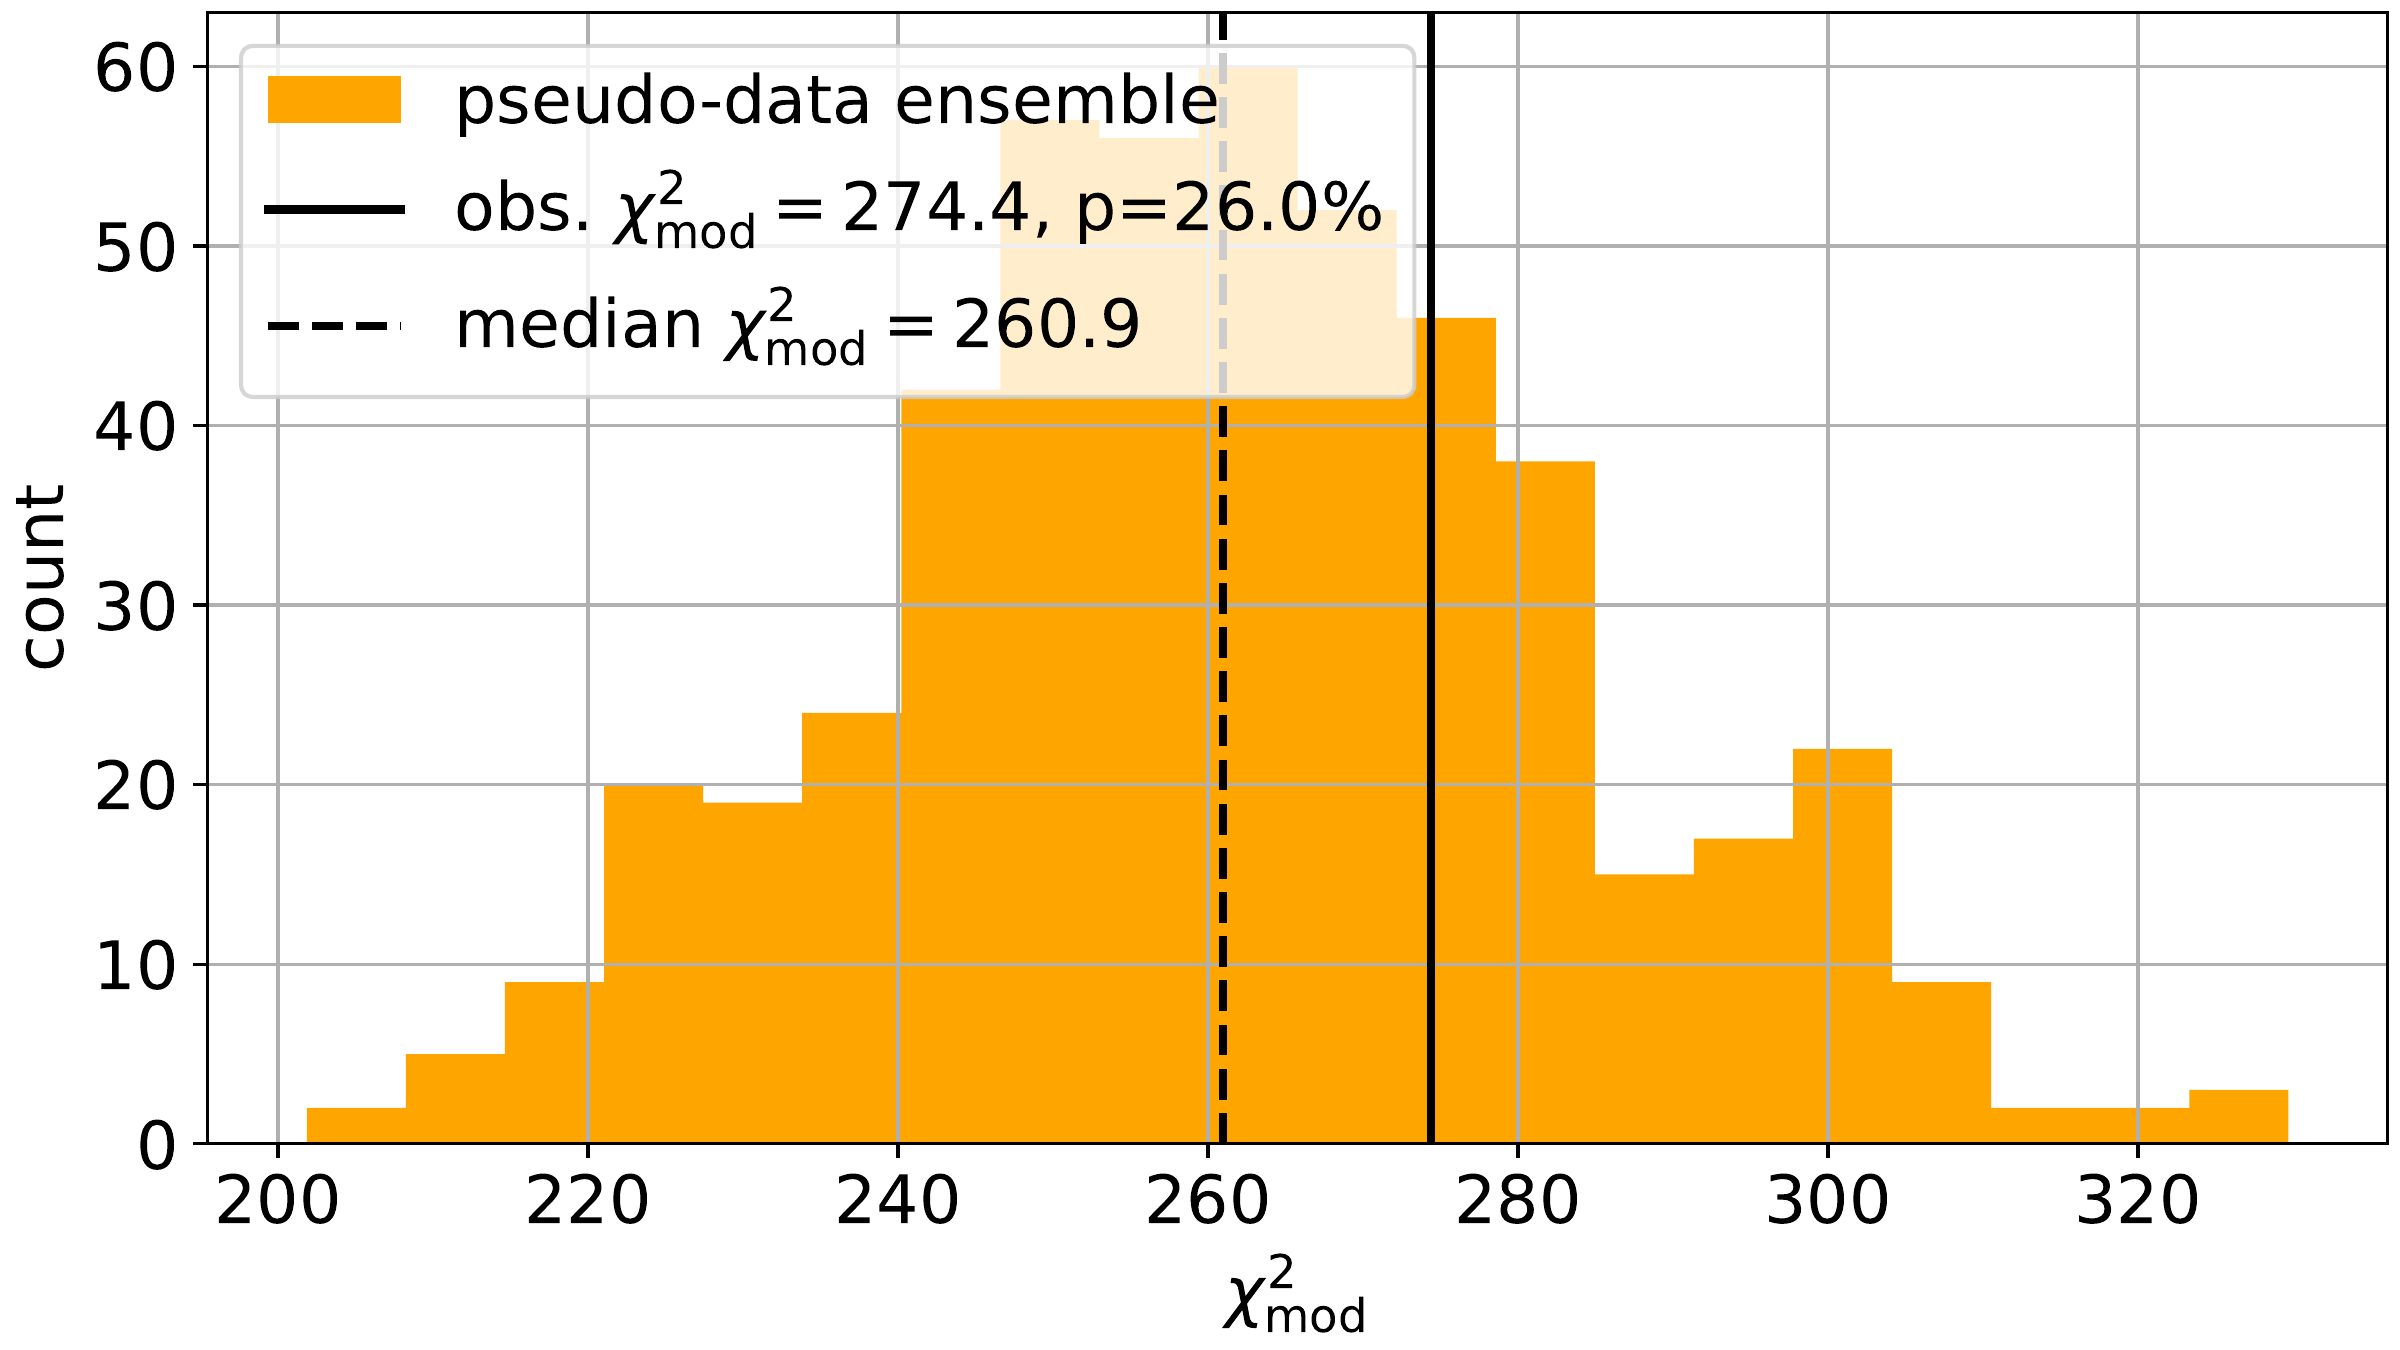
\includegraphics[width=0.49\linewidth]{figures/results/blind_fits/full_blind_fit_1.0_GeV_gauss_plus_poisson_step_3_4-1.png}
	\caption[Pseudo-data trials TS distribution (\SI{0.3}{\gev}, \SI{1.0}{\gev})]{Observed fit TS and TS distribution from pseudo-data trials for the \SI{0.3}{\gev} (left) and the \SI{1.0}{\gev} (right) mass set.}
    \labfig{pseudo_data_ensemble_appendix}
\end{figure*}


\setchapterstyle{lines}
\chapter{Analysis Results}
\labch{analysis_results}


\subsection{Best Fit Nuisance Parameters}

\begin{table*}
    \begin{tabular}{ ll lll lll }
    \hline\hline
    \textbf{Parameter} & \textbf{Nominal} & \multicolumn{3}{c}{\textbf{Best Fit}} & \multicolumn{3}{c}{\textbf{Nominal - Best Fit}} \\ 
    & & \textbf{0.3 GeV} & \textbf{0.6 GeV} &  \textbf{1.0 GeV} & \textbf{0.3 GeV} & \textbf{0.6 GeV} &  \textbf{1.0 GeV} \\ 
    \hline\hline
    $\Delta \gamma_\nu$ & 0.000000  & $-$0.007927 & $-$0.007957 & $-$0.006622 & 0.007927  & 0.007957  & 0.006622  \\
    $\rm{Barr} \; h_{\pi^+}$ & 0.000000  & $-$0.147462 & $-$0.147422 & $-$0.148043 & 0.147462  & 0.147422  & 0.148043  \\
    $\rm{Barr} \; i_{\pi^+}$ & 0.000000  & 0.475480  & 0.475323  & 0.520716  & $-$0.475480 & $-$0.475323 & $-$0.520716 \\
    $\rm{Barr} \; y_{K^+}$ & 0.000000  & 0.076161  & 0.076259  & 0.057927  & $-$0.076161 & $-$0.076259 & $-$0.057927 \\
    $\theta_{23} [\si{\degree}]$ & 47.504700 & 48.117259 & 48.118713 & 48.013150 & $-$0.612559 & $-$0.614013 & $-$0.508450 \\
    $\Delta m^{2}_{31} [\si{\electronvolt^2}]$ & 0.002475  & 0.002454  & 0.002454  & 0.002455  & 0.000020  & 0.000020  & 0.000019  \\
    $\rm{DIS}$ & 0.000000  & $-$0.248768 & $-$0.248845 & $-$0.216247 & 0.248768  & 0.248845  & 0.216247  \\
    $N_{\nu}$ & 1.000000  & 0.889145  & 0.889127  & 0.889543  & 0.110855  & 0.110873  & 0.110457  \\
    % $|U_{\tau 4}|^2$ & 0.000000  & 0.003017  & 0.000169  & 0.104056  & $-$0.003017 & $-$0.000169 & $-$0.104056 \\
    $\epsilon_{\rm{DOM}}$ & 1.000000  & 1.021987  & 1.022017  & 1.016791  & $-$0.021987 & $-$0.022017 & $-$0.016791 \\
    $\rm{hole \, ice} \; p_0$ & 0.101569  & $-$0.161352 & $-$0.161260 & $-$0.160133 & 0.262921  & 0.262829  & 0.261702  \\
    $\rm{hole \, ice} \; p_1$ & $-$0.049344 & $-$0.073700 & $-$0.073682 & $-$0.076212 & 0.024356  & 0.024338  & 0.026868  \\
    $\rm{ice \, absorption}$ & 1.000000  & 0.943262  & 0.943271  & 0.942023  & 0.056738  & 0.056729  & 0.057977  \\
    $\rm{ice \, scattering}$ & 1.050000  & 0.986150  & 0.986131  & 0.989374  & 0.063850  & 0.063869  & 0.060626  \\
    $N_\rm{bfr}$ & 0.000000  & 0.746674  & 0.746852  & 0.736461  & $-$0.746674 & $-$0.746852 & $-$0.736461 \\
    $M_\rm{A,QE}$ & 0.000000  & $-$0.170430 & $-$0.170677 & $-$0.121335 & 0.170430  & 0.170677  & 0.121335  \\
    $M_\rm{A,res}$ & 0.000000  & $-$0.125908 & $-$0.126076 & $-$0.071727 & 0.125908  & 0.126076  & 0.071727 \\
    \hline
    \end{tabular}
\caption[xx]{xx}
\labtab{best_fit_parameters}
\end{table*}
\todo{sort these by type of nuisance parameter?}



\subsection{Best Fit Parameters and Limits}

\begin{figure*}[h]
    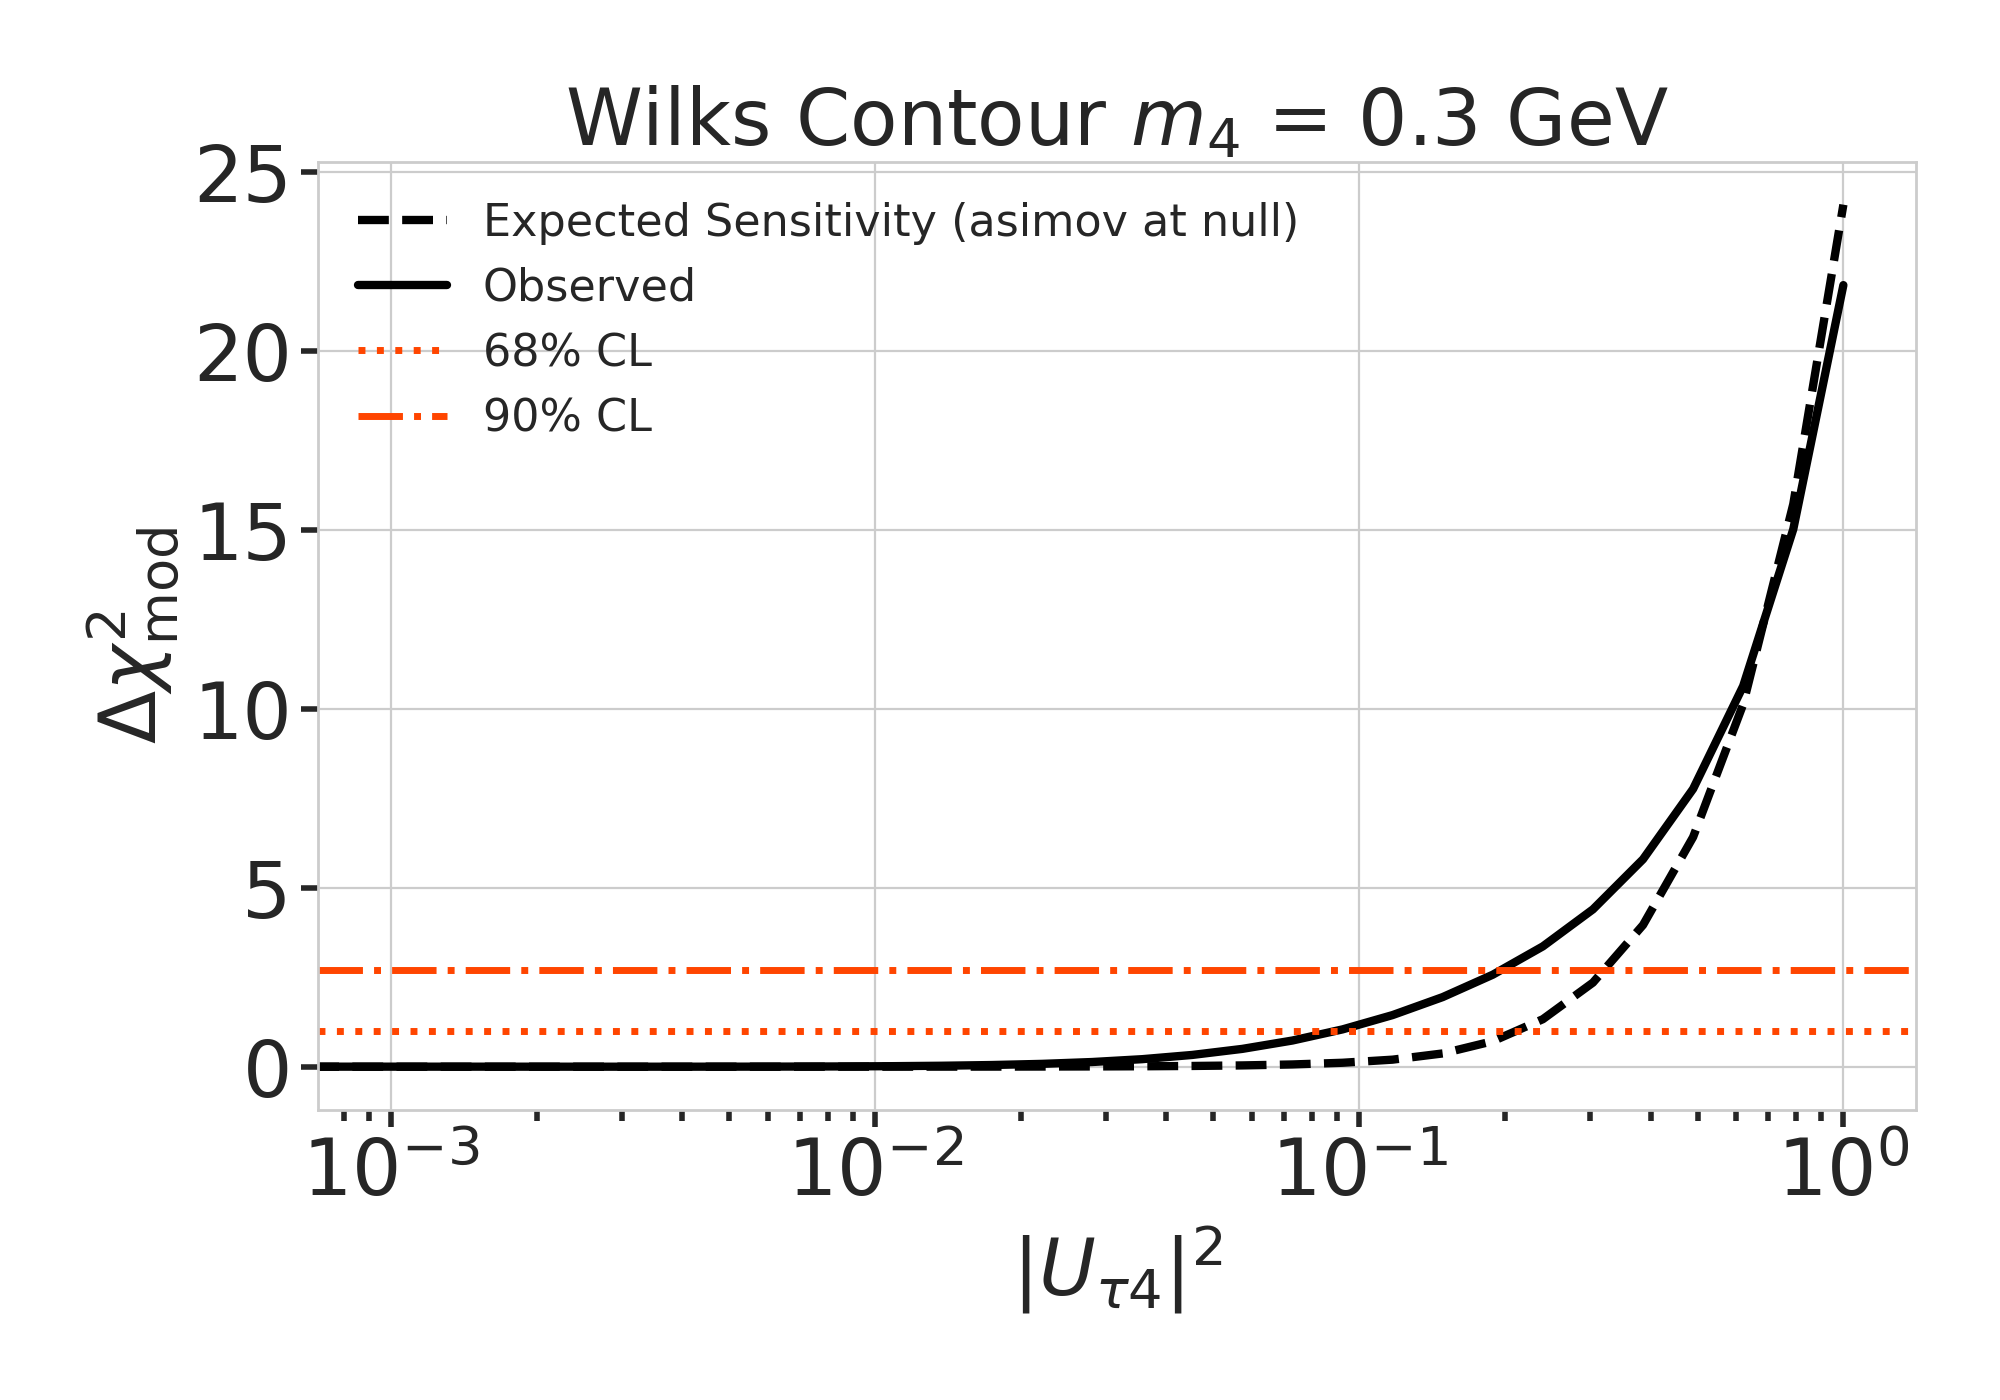
\includegraphics[width=0.49\linewidth]{figures/results/best_fit/sensitivity_and_wilks_scan_0.3_GeV_with_1sigma.png}
    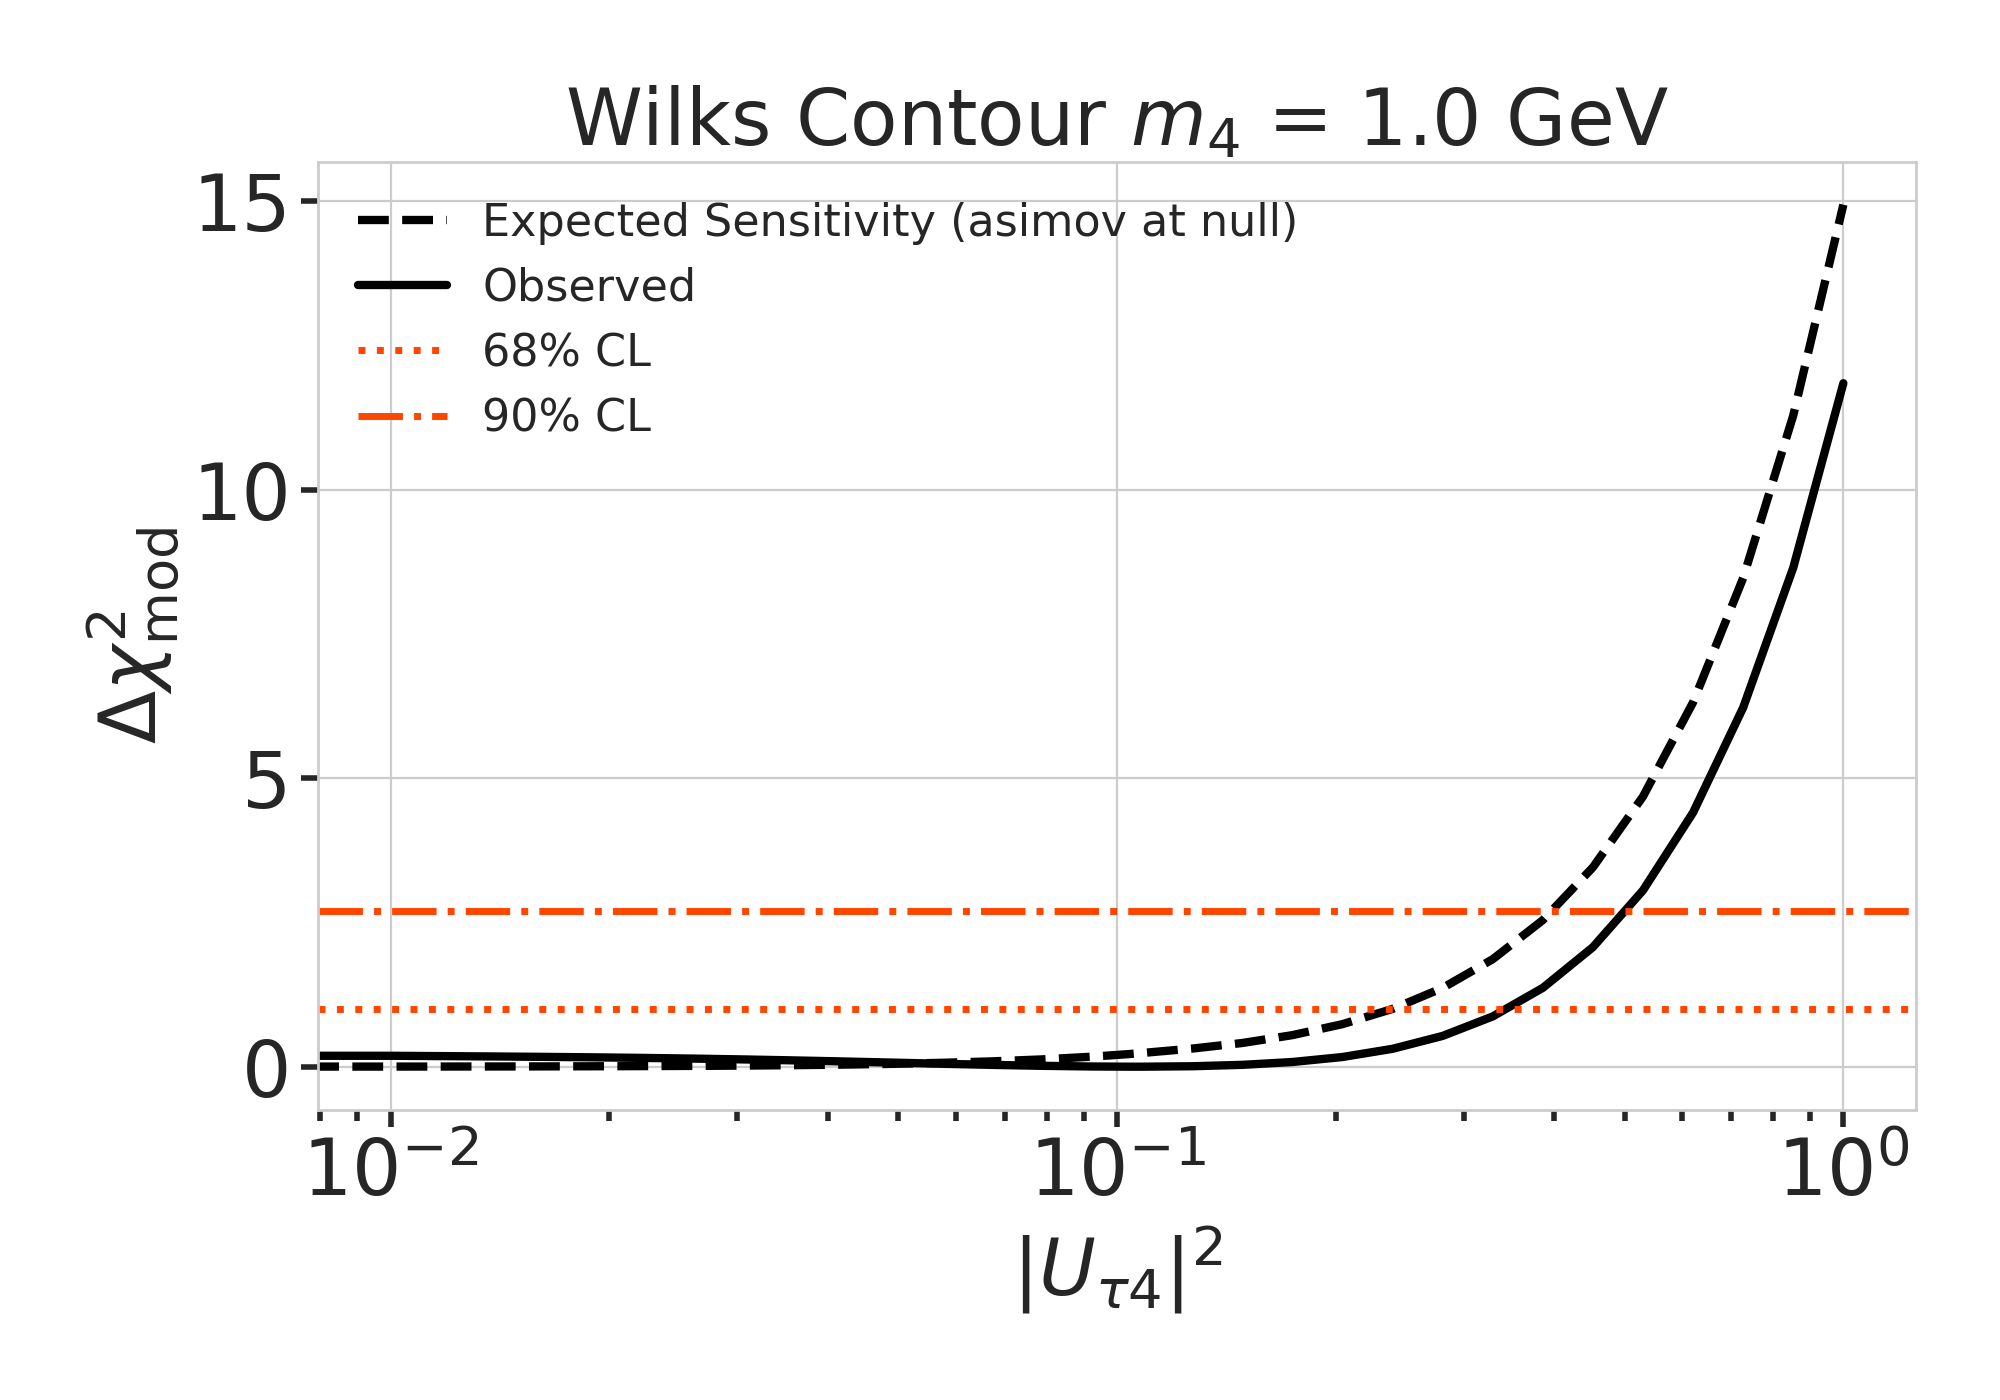
\includegraphics[width=0.49\linewidth]{figures/results/best_fit/sensitivity_and_wilks_scan_1.0_GeV_with_1sigma.png}
	\caption[xx]{xx}
    \labfig{brazil_bands_appendix}
\end{figure*}

